\chapter{Experiments and Results}
\label{ch:results}

This chapter presents comprehensive experimental results comparing eight INR architectures on 3D occupancy reconstruction using the Nefertiti bust mesh. We analyze quantitative metrics, examine the relationship between architectural properties and performance, evaluate computational efficiency, and characterize failure modes.

\section{Experimental Setup}
\label{sec:setup}

Our experiments evaluate all eight INR methods on the Nefertiti bust mesh, a high-resolution cultural heritage scan featuring smooth facial geometry, fine ornamental details on the crown, and sharp geometric transitions between the face and headdress. This mesh provides a challenging test for fine detail reconstruction while remaining computationally tractable for systematic comparison.

The mesh is normalized to $[-1, 1]^3$ and sampled once, ahead of training, into a fixed dataset of 500,000 labelled points: half drawn uniformly from the bounding box and half drawn near the surface with Gaussian displacement of standard deviation $\sigma = 0.01$. This gives the network training signal near boundaries, where classification is most difficult, while also teaching the global occupancy structure. Because the dataset is fixed rather than resampled each epoch, the same points are revisited throughout training.

All models share the same depth and width: 3-dimensional input $(x, y, z)$, 4 hidden layers with 256 features each, and 1-dimensional output. Matching depth and width does not match capacity, however: parameter counts range from 133{,}250 (FR) to 1{,}057{,}282 (WIRE), with most methods near 265{,}000. We return to this confound when interpreting the results. Training proceeds for 500 epochs with batch size 16,384 and initial learning rate $1 \times 10^{-4}$ following cosine annealing to $1 \times 10^{-6}$. Two methods required learning rate overrides for stable convergence: GAUSS used $1 \times 10^{-3}$ and MFN used $3 \times 10^{-4}$. Binary Cross-Entropy loss is used throughout, with gradient clipping at maximum norm 1.0.

The dataset is split into 450,000 training points and 50,000 validation points by a seeded generator, so every method is evaluated on the same held-out points. Evaluation IoU is computed on that held-out split; Chamfer-L1 and normal consistency are computed from a mesh extracted by Marching Cubes on a dense $256^3$ grid (16,777,216 points). All experiments were conducted on a single NVIDIA Tesla T4 GPU using PyTorch 2.0 with CUDA 11.8.

\section{Quantitative Results on Nefertiti Bust}

We ran each configuration over four random seeds, differing in weight initialization and batch-shuffling order; the train/validation split is held fixed across seeds, so every run is scored on the same 50,000 held-out points. Table~\ref{tab:seed_results} reports the mean and standard deviation of each metric, and Figure~\ref{fig:iou_error_bars} plots evaluation IoU with error bars. Evaluation IoU is measured on the held-out split at threshold $\tau = 0.5$; the surface metrics are measured on the $256^3$ marching-cubes reconstruction.

% Table generated from results_3d_seeds.csv by aggregate_seeds.py -- do not edit by hand.
% AUTO-GENERATED by aggregate_seeds.py -- do not edit by hand.
\begin{table}[htbp]
\centering
\caption{Evaluation IoU over 4 seeds (mean $\pm$ standard deviation), ranked by mean. Methods in the leading cluster --- those a Holm-corrected Welch $t$-test cannot separate from the best --- are marked $\dagger$. Chamfer-L1 and normal consistency are seed means.}
\label{tab:seed_results}
\begin{tabular}{lccc}
\toprule
\textbf{Method} & \textbf{Eval IoU (mean $\pm$ std)} $\uparrow$ & \textbf{Chamfer-L1} $\downarrow$ & \textbf{Normal Cons.} $\uparrow$ \\
\midrule
Fourier Features$^\dagger$ & \textbf{0.9677 $\pm$ 0.0009} & 0.011014 & 0.9796 \\
INCODE$^\dagger$ & 0.9674 $\pm$ 0.0022 & 0.010955 & 0.9808 \\
SIREN & 0.9562 $\pm$ 0.0024 & 0.010946 & 0.9799 \\
FR & 0.9562 $\pm$ 0.0020 & 0.010977 & 0.9811 \\
FINER & 0.9545 $\pm$ 0.0016 & 0.010954 & 0.9792 \\
WIRE & 0.9525 $\pm$ 0.0032 & 0.010972 & 0.9796 \\
MFN & 0.9320 $\pm$ 0.0012 & 0.011070 & 0.9782 \\
GAUSS & 0.9148 $\pm$ 0.0082 & 0.011224 & 0.9756 \\
\bottomrule
\end{tabular}
\end{table}


\begin{figure}[htbp]
\centering
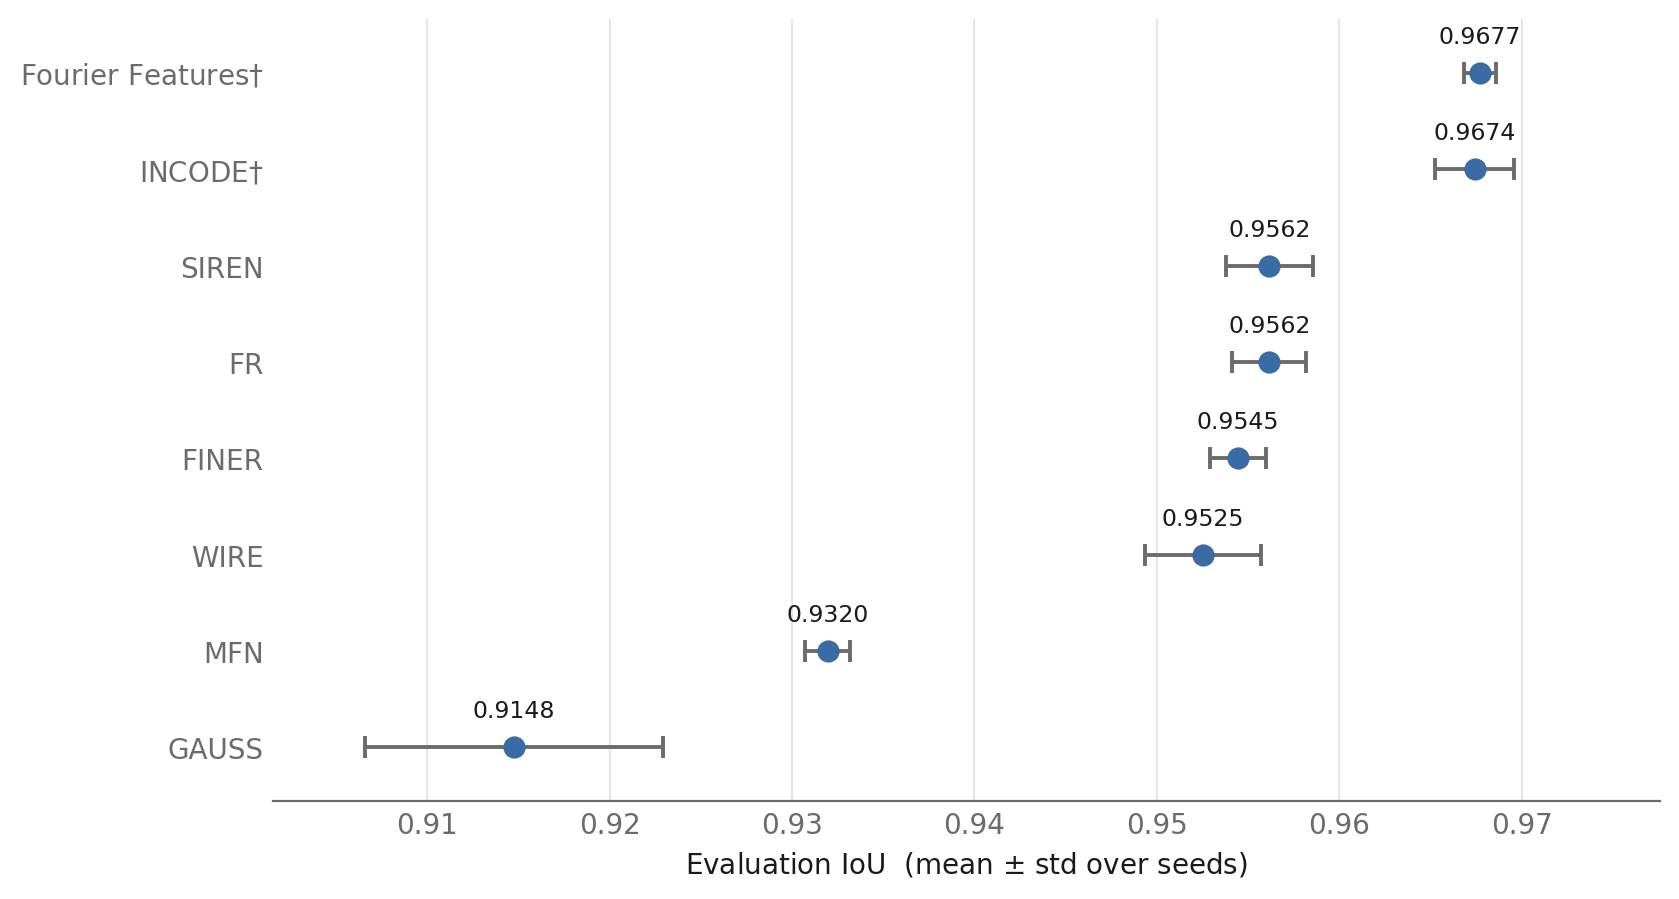
\includegraphics[width=0.92\textwidth]{Figures/results/iou_error_bars.png}
\caption{Evaluation IoU per method (mean over four seeds; error bars $\pm$ one standard deviation), sorted by mean. Methods marked $\dagger$ form the leading cluster that a Holm-corrected Welch $t$-test cannot separate from the best. Fourier Features and INCODE sit clearly above a middle group of four; MFN and GAUSS trail, and GAUSS shows by far the largest run-to-run spread.}
\label{fig:iou_error_bars}
\end{figure}

Two methods form a distinct top tier: Fourier Features ($0.9677 \pm 0.0009$) and INCODE ($0.9674 \pm 0.0022$). They are statistically indistinguishable from each other but significantly ahead of every other method. % AUTO-GENERATED by aggregate_seeds.py
A one-way ANOVA across the 8 methods rejects equality of means ($F=108.61$, $p=1.3e-16$). Holm-corrected Welch $t$-tests of the best method against each other place 2 methods in a leading cluster that cannot be separated at $\alpha=0.05$: Fourier Features, INCODE.


Below them sits a middle group --- SIREN and FR (both $0.9562$), FINER ($0.9545$), and WIRE ($0.9525$) --- separated from the top tier by roughly 1.1 percentage points. The seeds resolve this gap cleanly precisely because the per-method standard deviations are small (0.0009--0.0032): the separation is an order of magnitude larger than the noise. MFN ($0.9320 \pm 0.0012$) and GAUSS ($0.9148 \pm 0.0082$) trail by a further 2--4 points, and GAUSS's spread is the largest of any method, consistent with the unstable optimization examined in Section~\ref{sec:dynamics}.

The surface metrics broadly track the IoU ordering: GAUSS has the worst Chamfer-L1 and normal consistency, and the top tier the best. Because the surface samples underlying both metrics are drawn without a fixed seed, we do not read into differences at the fourth decimal place.

Notably, the top tier pairs one frequency-compact method (INCODE) with one lacking the property (Fourier Features), which we return to in Section~\ref{sec:properties}.

Finally, the Fourier Features figures above use a frequency scale $\sigma = 1.0$. The same architecture at $\sigma = 10.0$ collapses to an evaluation IoU of 0.7966; we analyse this ablation in Section~\ref{sec:fourier_ablation}, as it isolates the effect of frequency scale more cleanly, and more dramatically, than any comparison across architectures.

\section{Qualitative Results}

Figure~\ref{fig:reconstruction_comparison} compares the ground-truth bust with a top-tier method (INCODE) and the weakest (GAUSS). Images are rendered at consistent viewpoint and lighting for fair comparison.

\begin{figure}[htbp]
\centering
\begin{subfigure}[b]{0.48\textwidth}
\centering
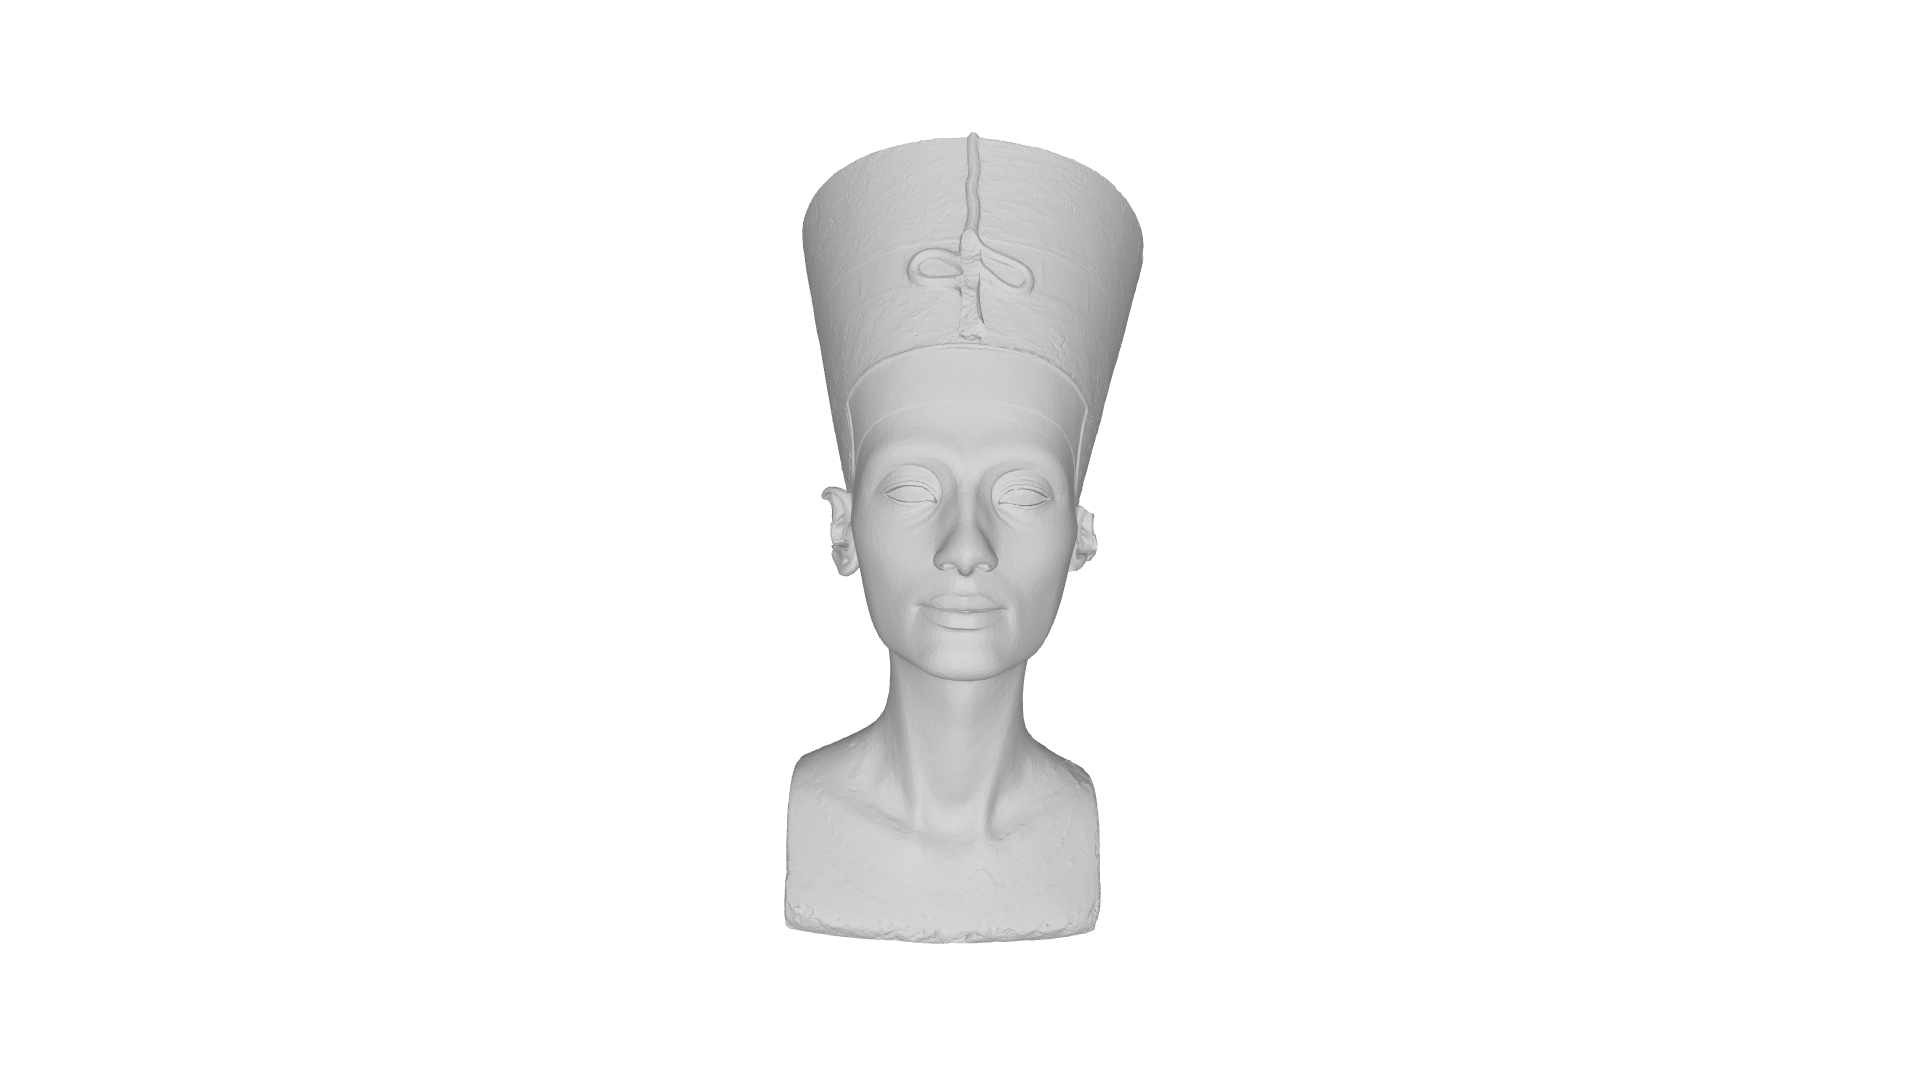
\includegraphics[width=\textwidth]{Figures/results/nefertiti_ground_truth.png}
\caption{Ground Truth}
\label{fig:gt}
\end{subfigure}
\hfill
\begin{subfigure}[b]{0.48\textwidth}
\centering
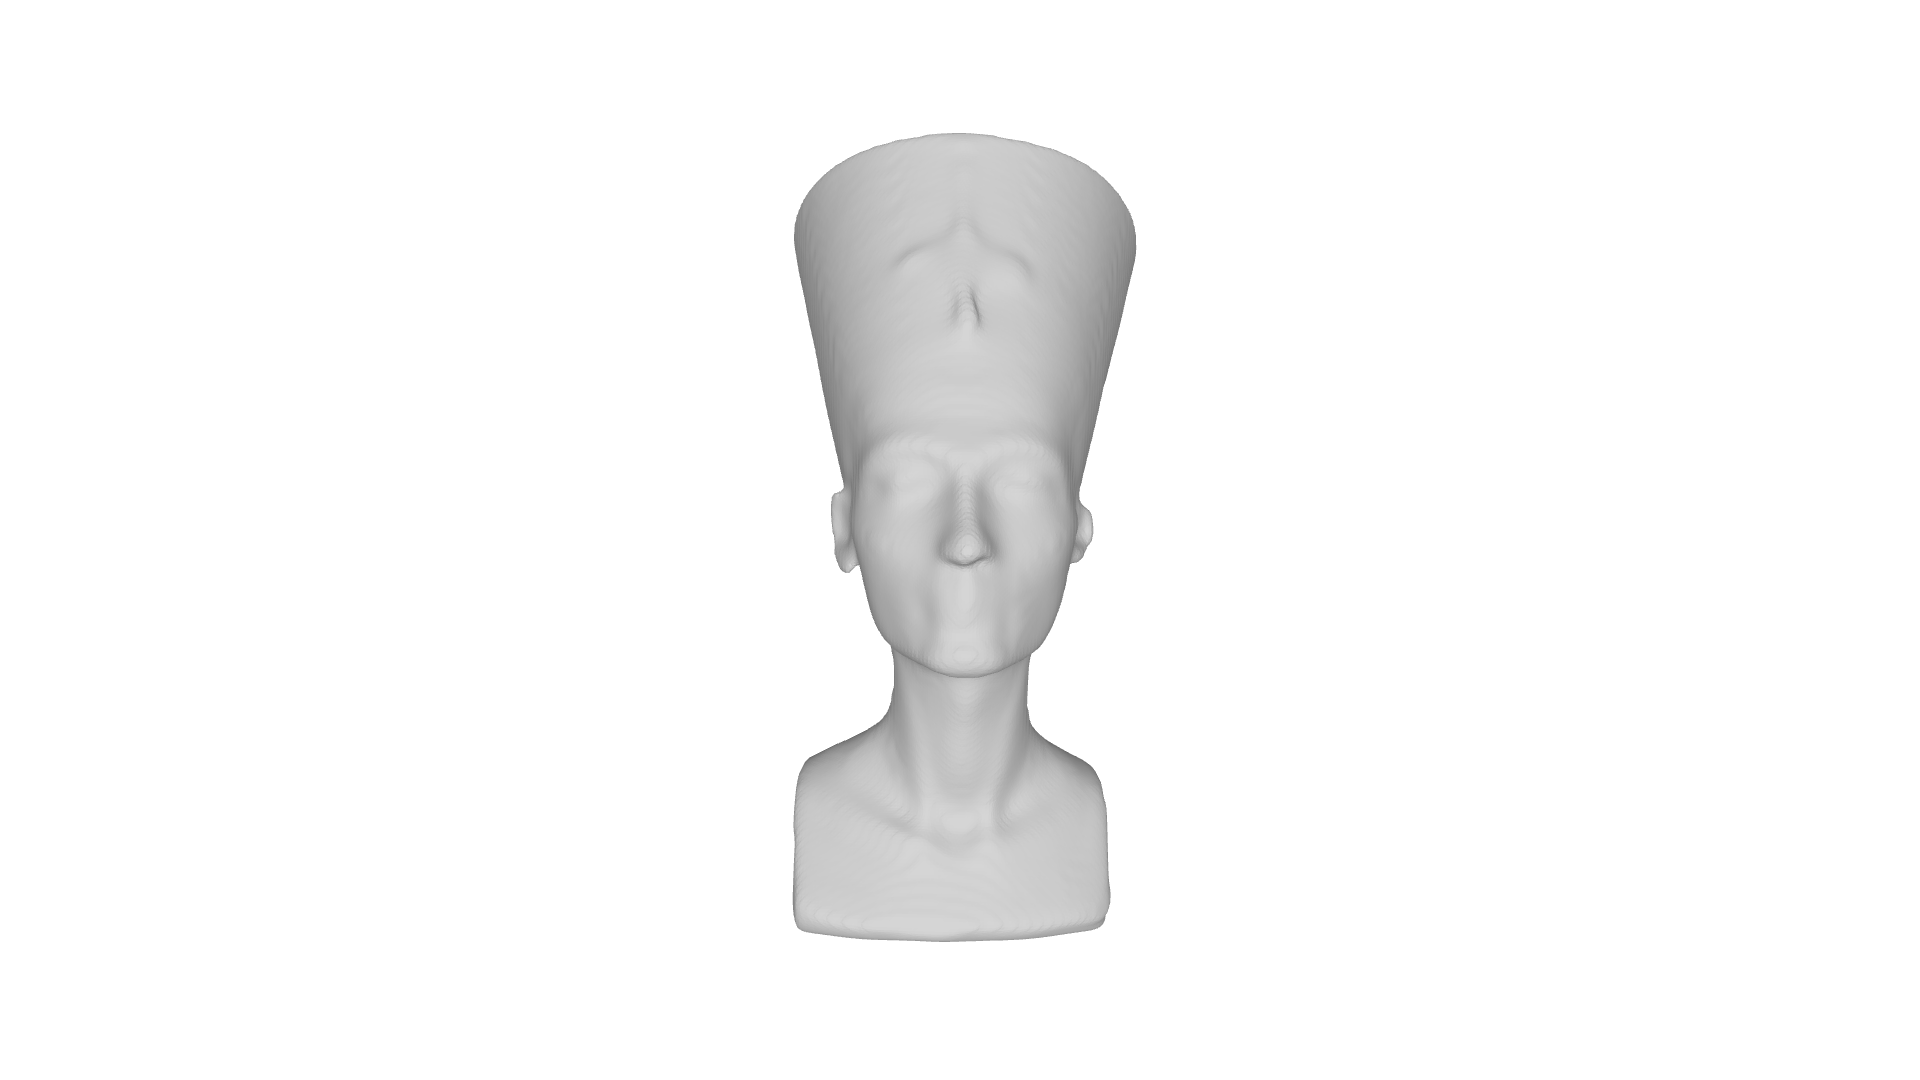
\includegraphics[width=\textwidth]{Figures/results/nefertiti_incode.png}
\caption{INCODE (mean IoU: 0.9674)}
\label{fig:incode}
\end{subfigure}

\vspace{0.3cm}

\begin{subfigure}[b]{0.48\textwidth}
\centering
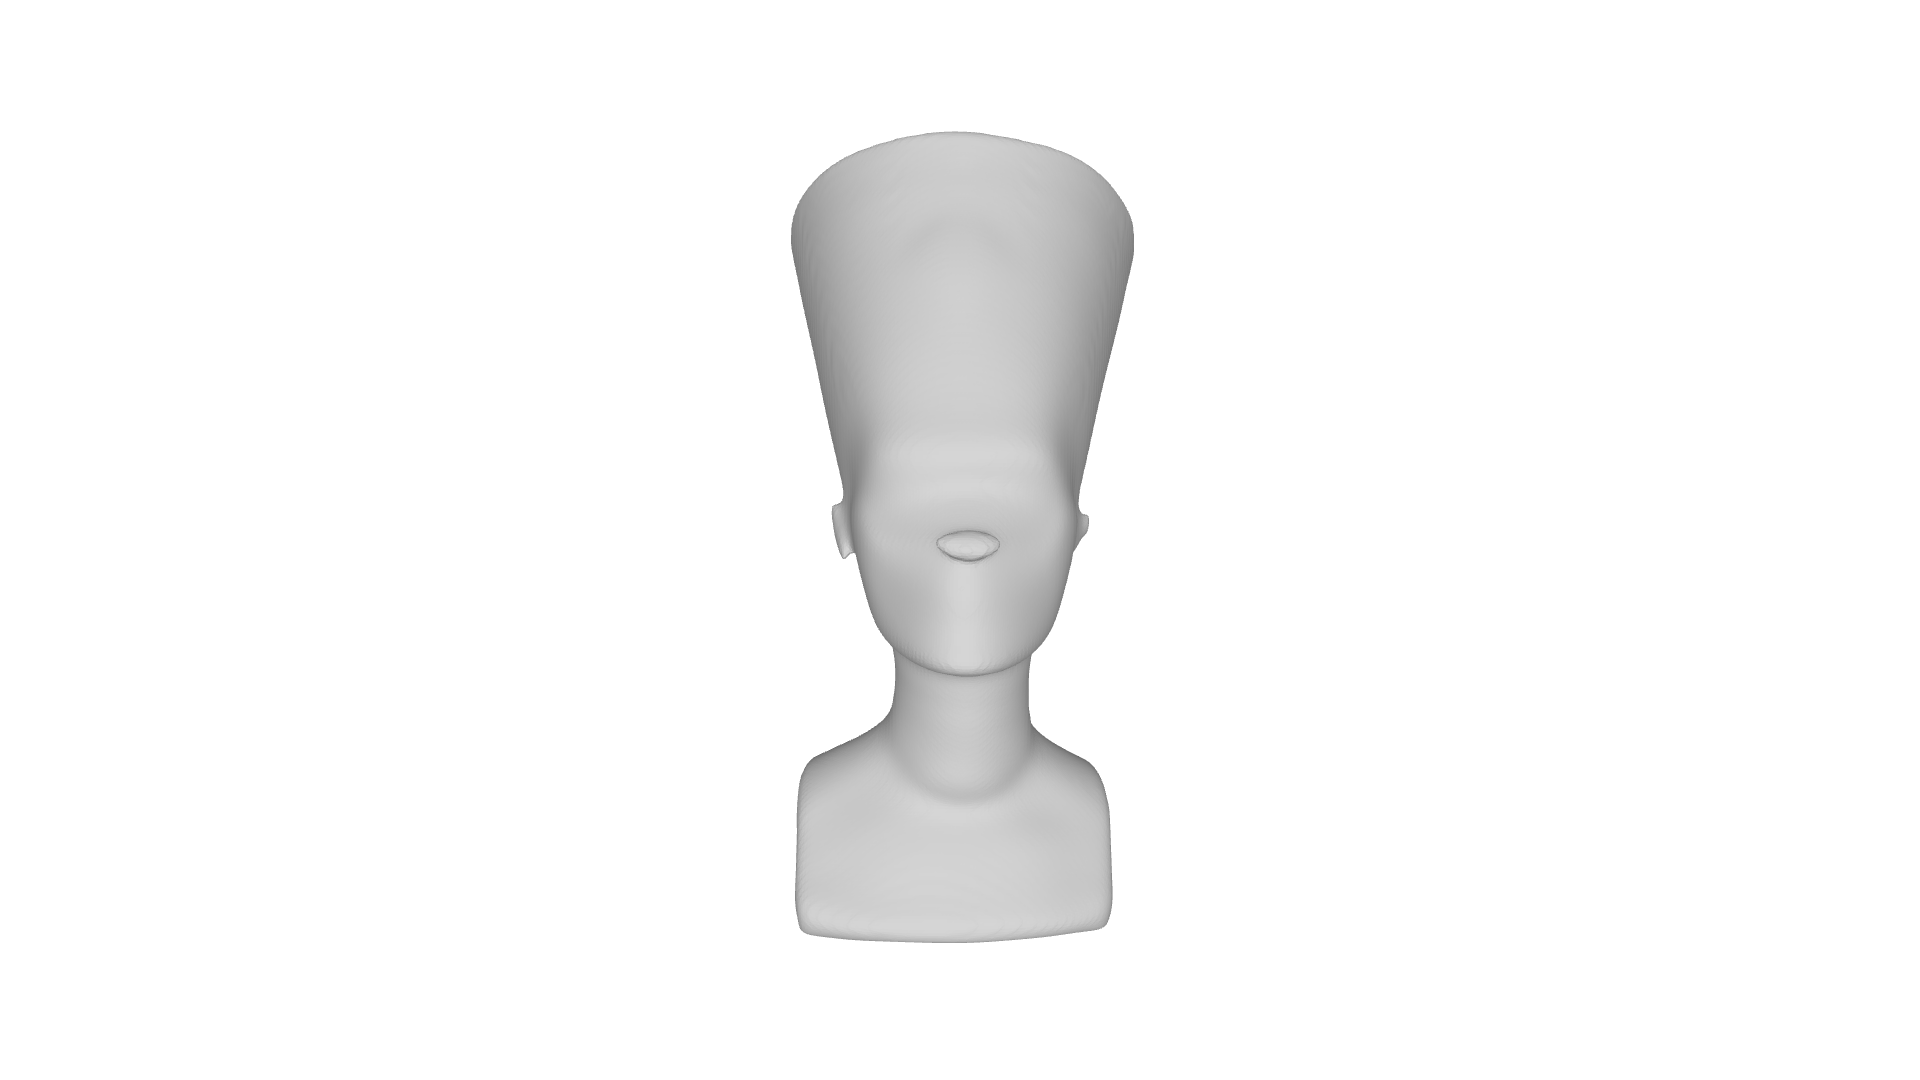
\includegraphics[width=\textwidth]{Figures/results/nefertiti_gauss.png}
\caption{GAUSS (mean IoU: 0.9148)}
\label{fig:gauss}
\end{subfigure}
\caption{Visual comparison of 3D occupancy reconstruction on the Nefertiti bust. INCODE recovers the silhouette and gross facial structure but loses the headdress band and most of the crown ornament. GAUSS smooths the face away almost entirely. All renders use identical camera position, lighting, and resolution ($1920 \times 1080$).}
\label{fig:reconstruction_comparison}
\end{figure}

The renders temper the quantitative picture considerably. An evaluation IoU above 0.95 sounds close to perfect, but IoU is dominated by the object's interior volume, which every method recovers easily; the surface detail that distinguishes a good reconstruction contributes very little to the score.

INCODE (Fig.~\ref{fig:incode}) recovers the silhouette, crown, neck, and shoulders faithfully, and the nose and brow ridge remain identifiable. Beyond that, detail is lost: the eyes become shallow depressions rather than defined lids, the lips are indistinct, the headdress band has disappeared, and the uraeus ornament survives only as a faint ridge. This is the \emph{best} reconstruction we obtained, and it does not preserve the fine ornamental detail that motivated the choice of this mesh. GAUSS (Fig.~\ref{fig:gauss}) is oversmoothing in its clearest form, consistent with a network that never fit the training data closely: the eyes are absent entirely and the crown is a featureless blob.

All methods lose the crown ornamentation and the headdress edge, differing mainly in how much facial structure survives. At this network size and training budget, none of the eight architectures resolves the detail this mesh was chosen to test.

Figure~\ref{fig:all_methods} presents reconstructions from all eight methods in a two-row grid, ordered by evaluation IoU.

\begin{figure}[htbp]
\centering
% Row 1: Top 4 methods
\begin{subfigure}[b]{0.24\textwidth}
\centering
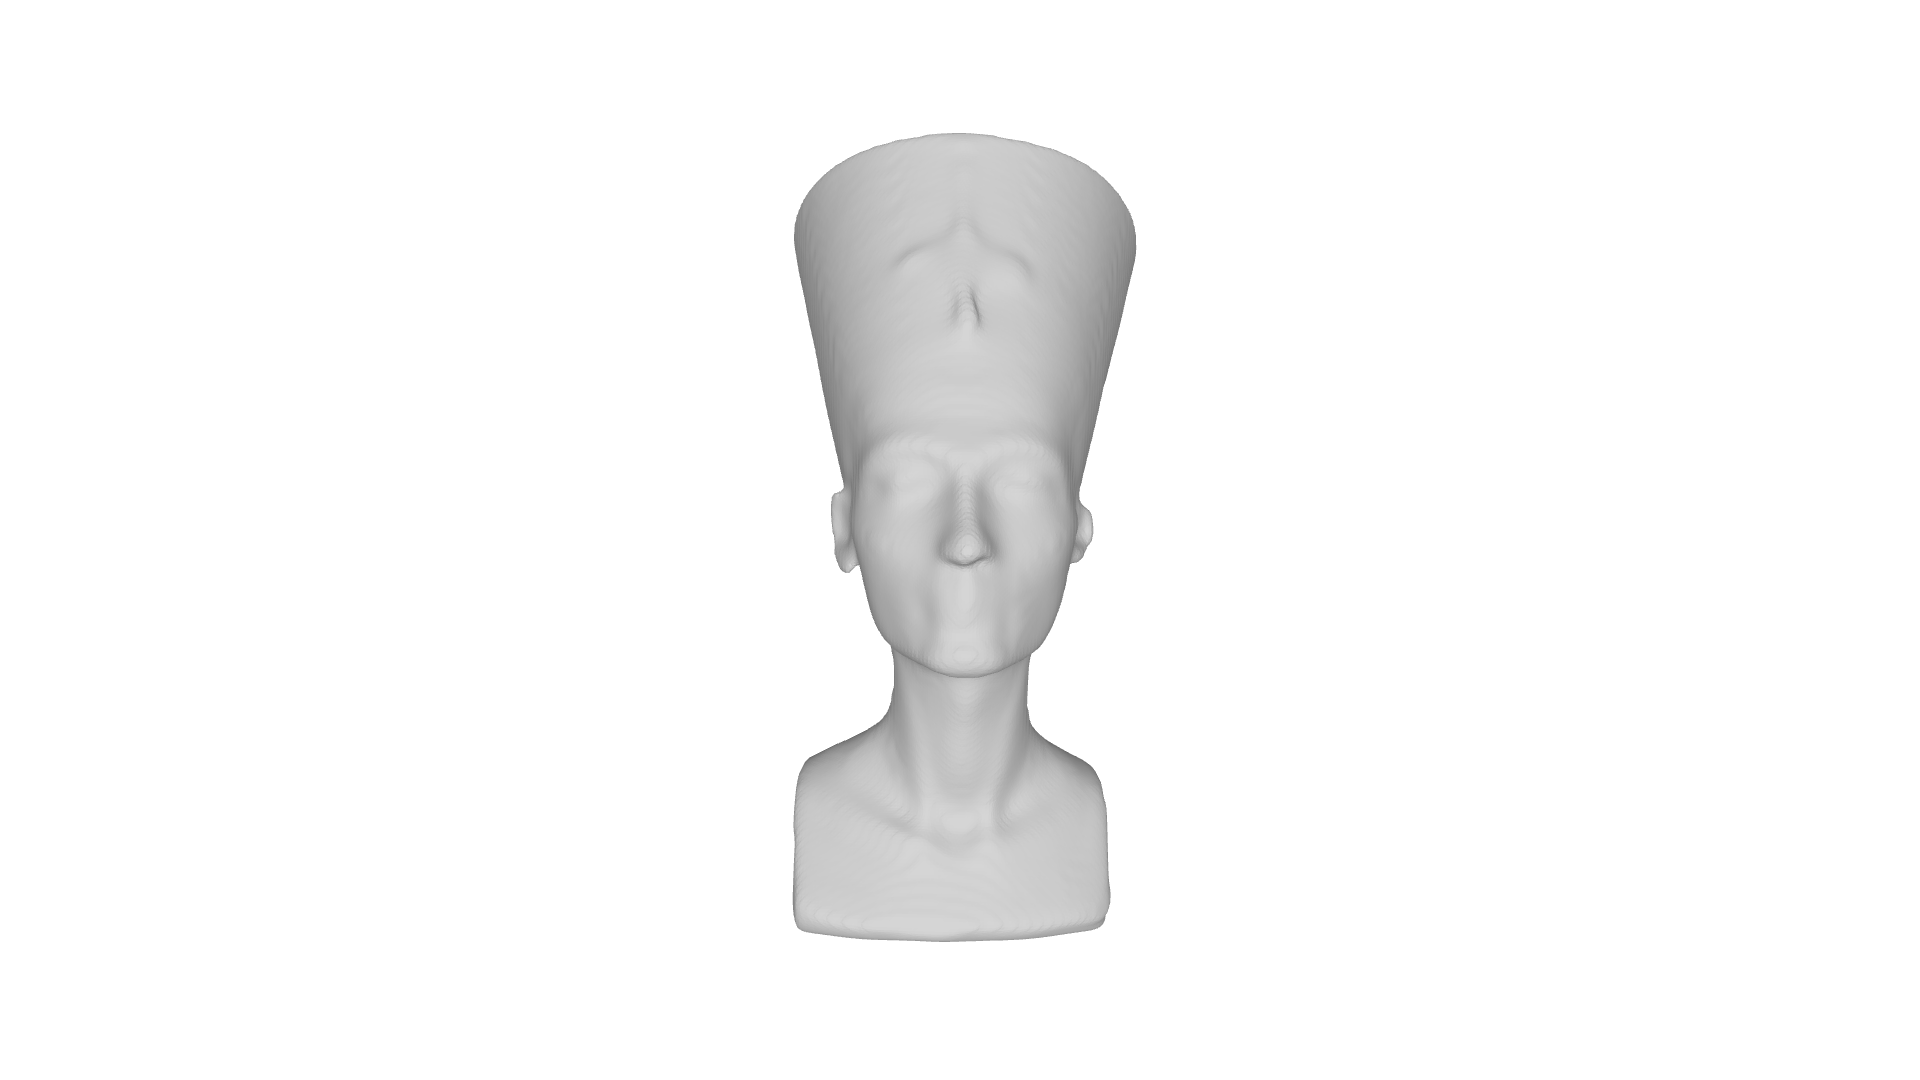
\includegraphics[width=\textwidth]{Figures/results/nefertiti_incode.png}
\caption{INCODE (0.9674)}
\end{subfigure}
\hfill
\begin{subfigure}[b]{0.24\textwidth}
\centering
% NOTE: requires the sigma=1.0 render. Re-render outputs_3d/fourier_nefertiti.obj
% from the corrected run; the sigma=10 image is kept as nefertiti_fourier_sigma10.png.
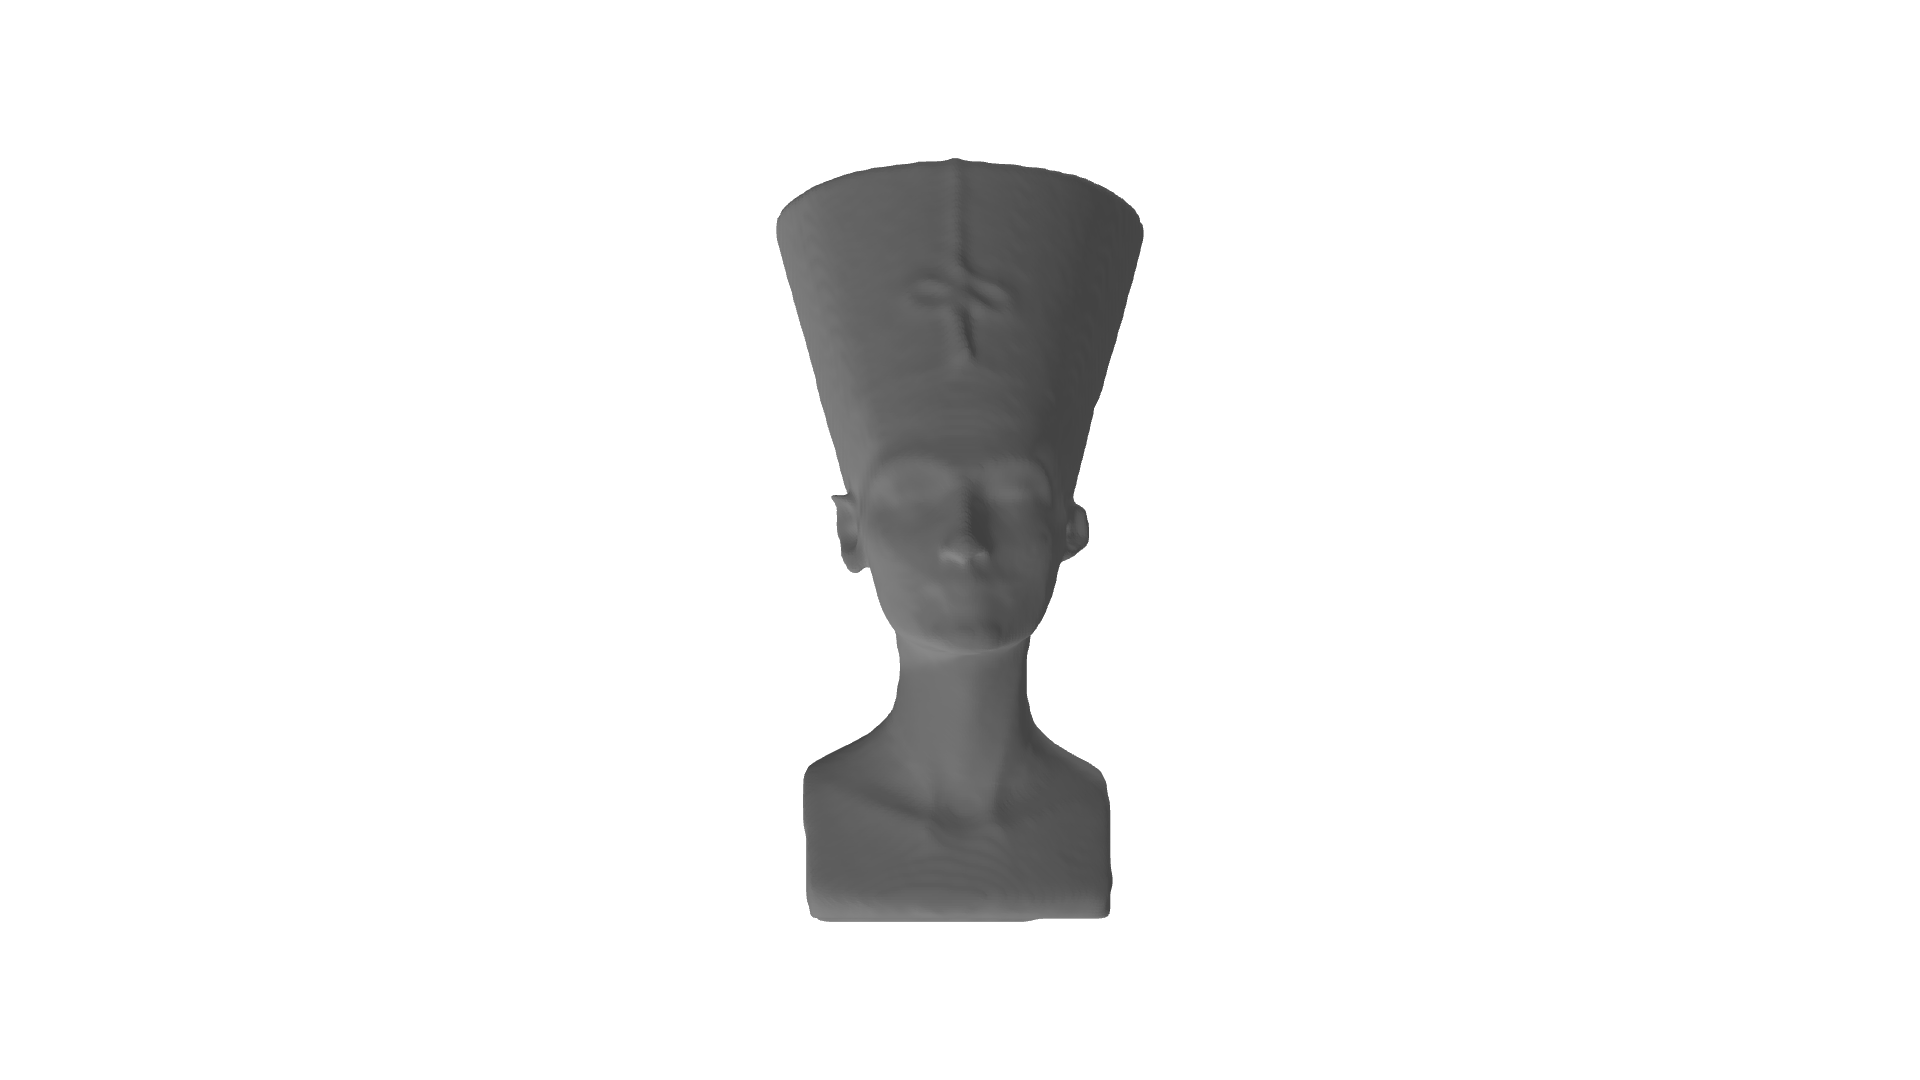
\includegraphics[width=\textwidth]{Figures/results/nefertiti_fourier.png}
\caption{Fourier (0.9677)}
\end{subfigure}
\hfill
\begin{subfigure}[b]{0.24\textwidth}
\centering
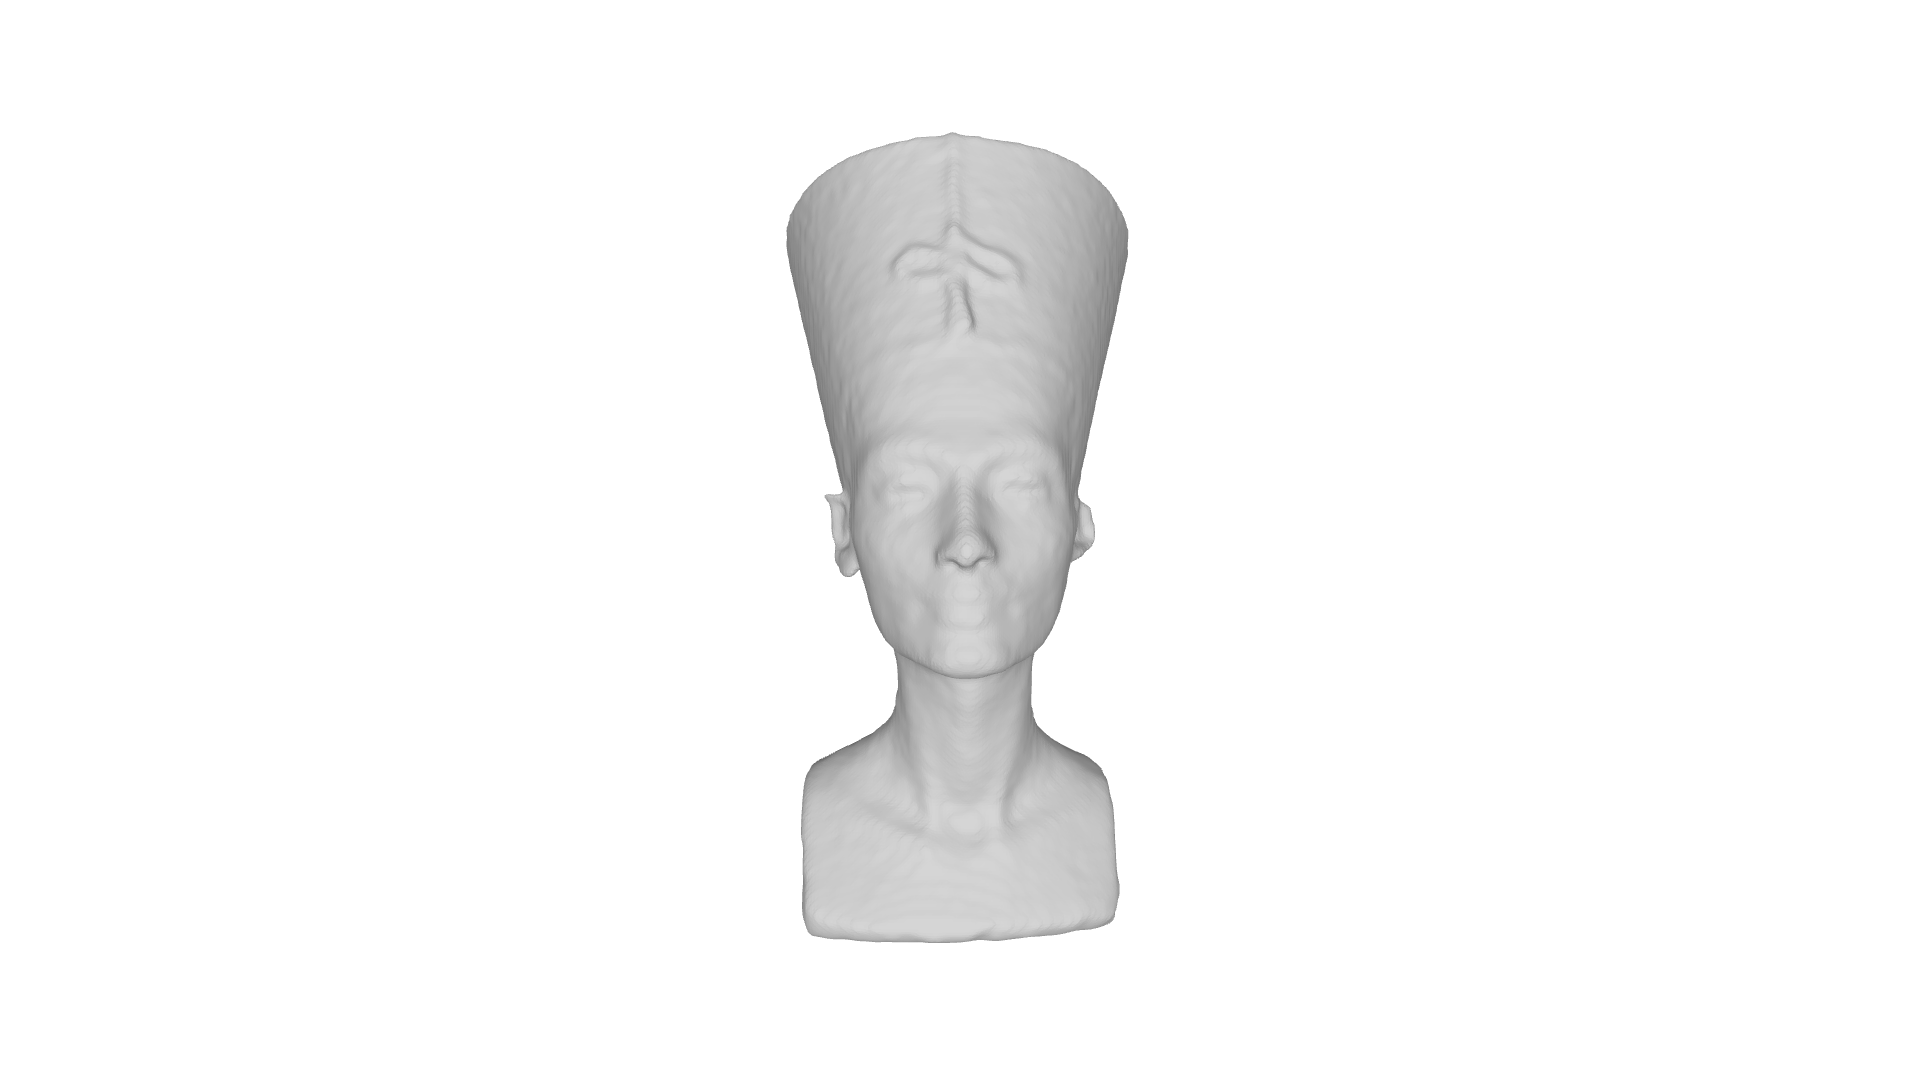
\includegraphics[width=\textwidth]{Figures/results/nefertiti_fr.png}
\caption{FR (0.9562)}
\end{subfigure}
\hfill
\begin{subfigure}[b]{0.24\textwidth}
\centering
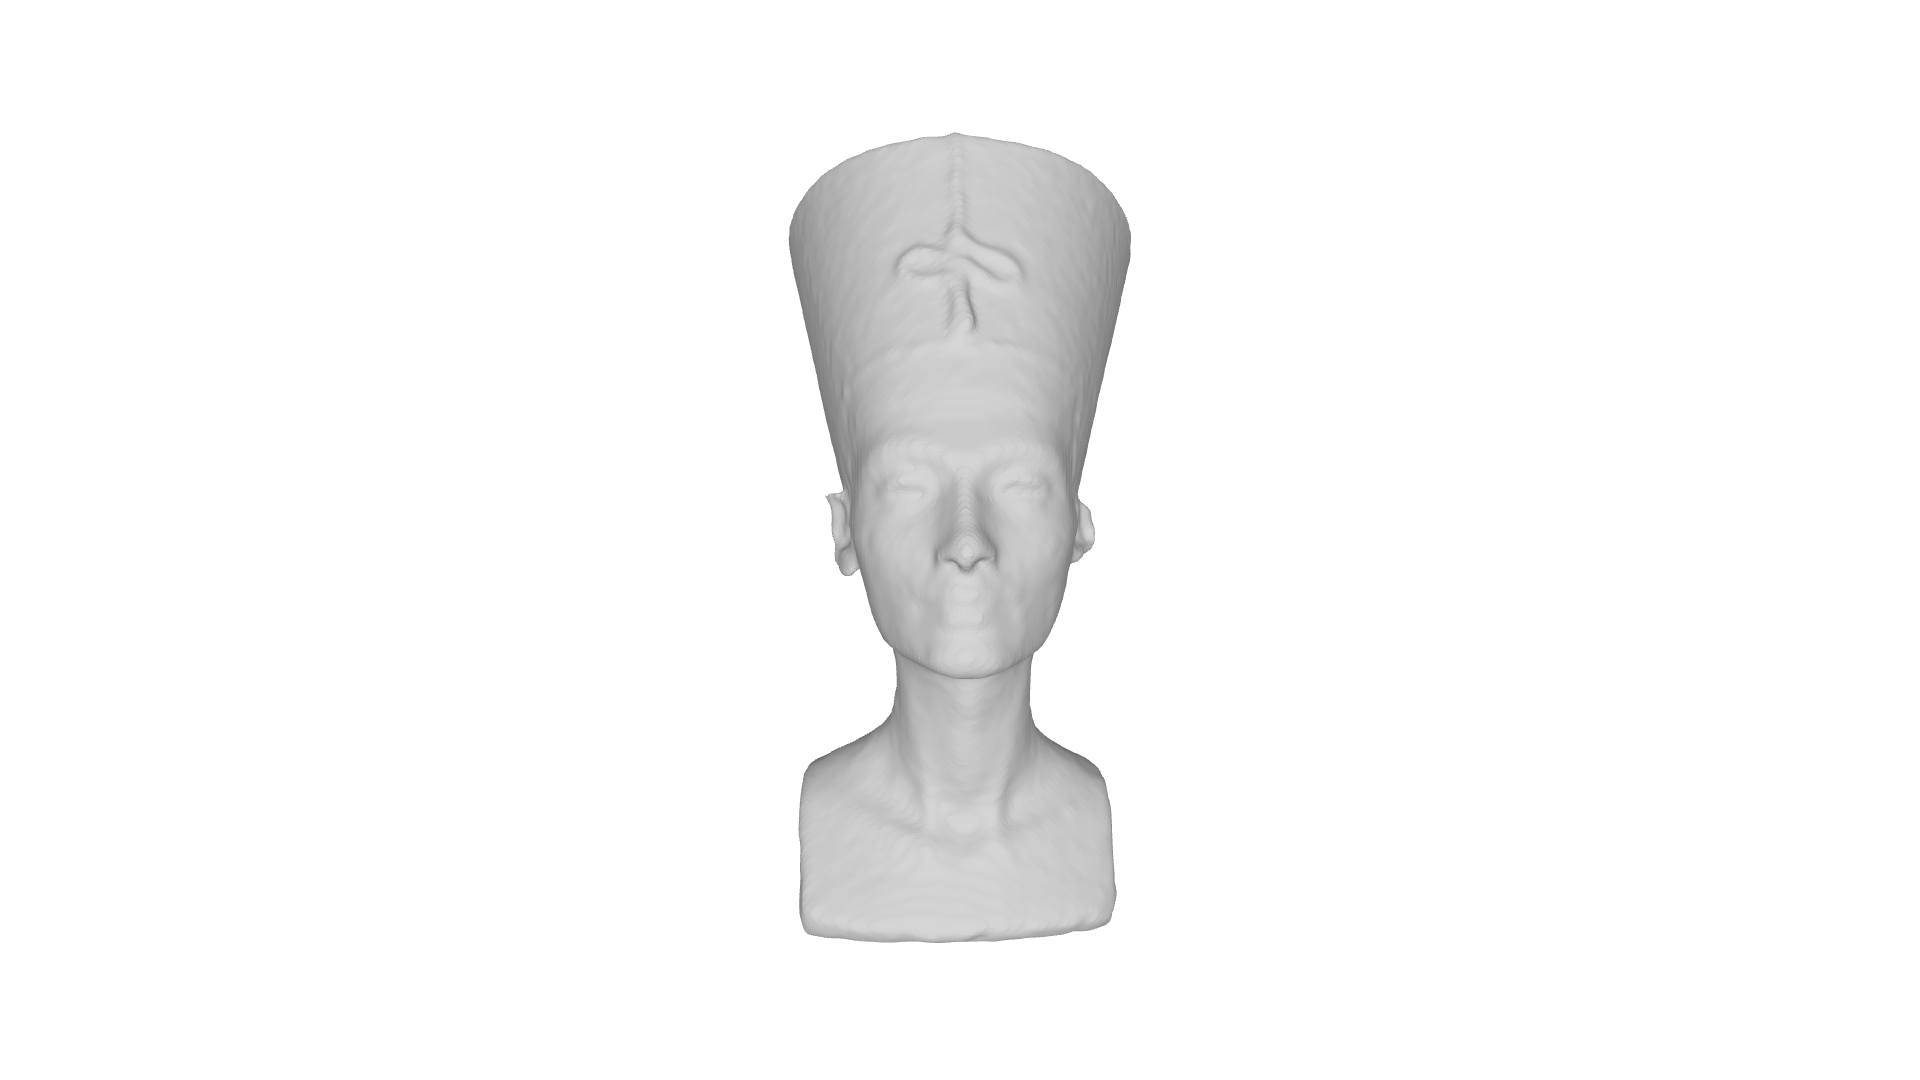
\includegraphics[width=\textwidth]{Figures/results/nefertiti_siren.png}
\caption{SIREN (0.9562)}
\end{subfigure}

\vspace{0.2cm}

% Row 2: remaining methods
\begin{subfigure}[b]{0.24\textwidth}
\centering
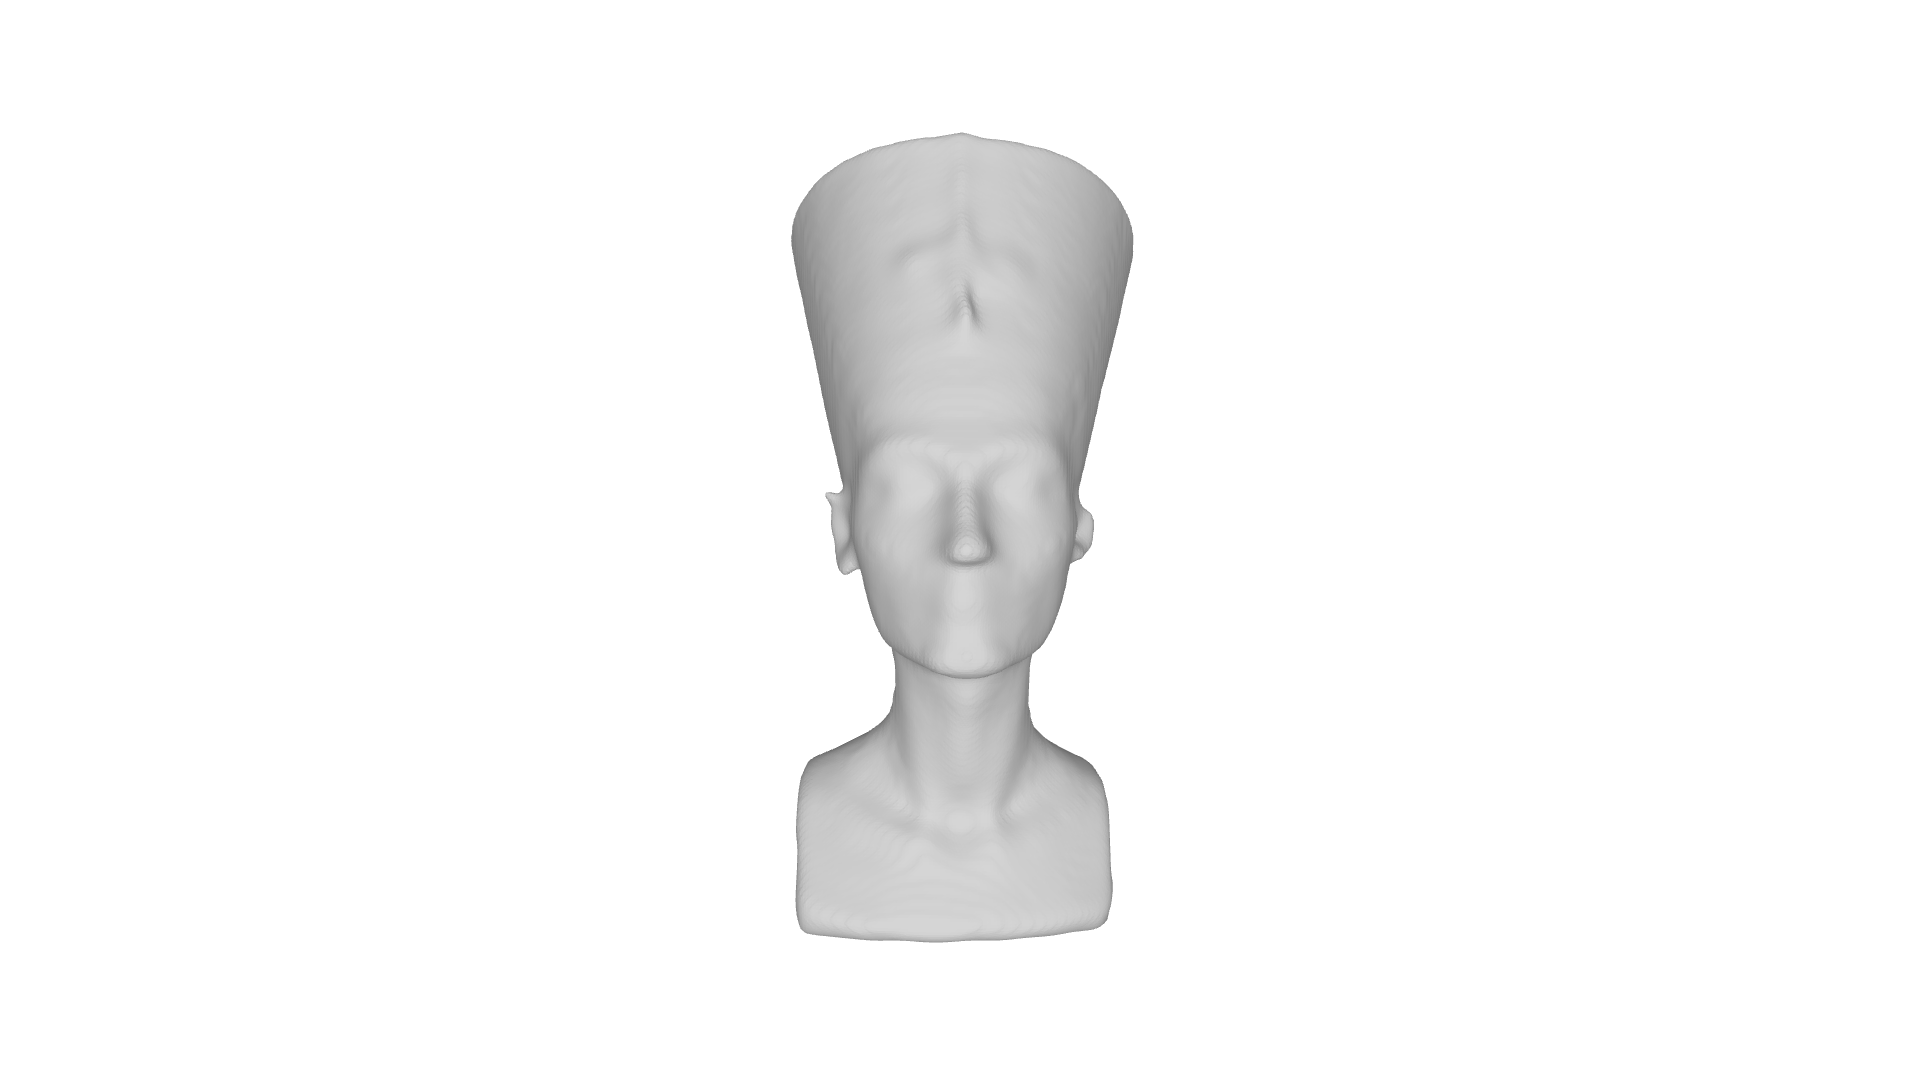
\includegraphics[width=\textwidth]{Figures/results/nefertiti_finer.png}
\caption{FINER (0.9545)}
\end{subfigure}
\hfill
\begin{subfigure}[b]{0.24\textwidth}
\centering
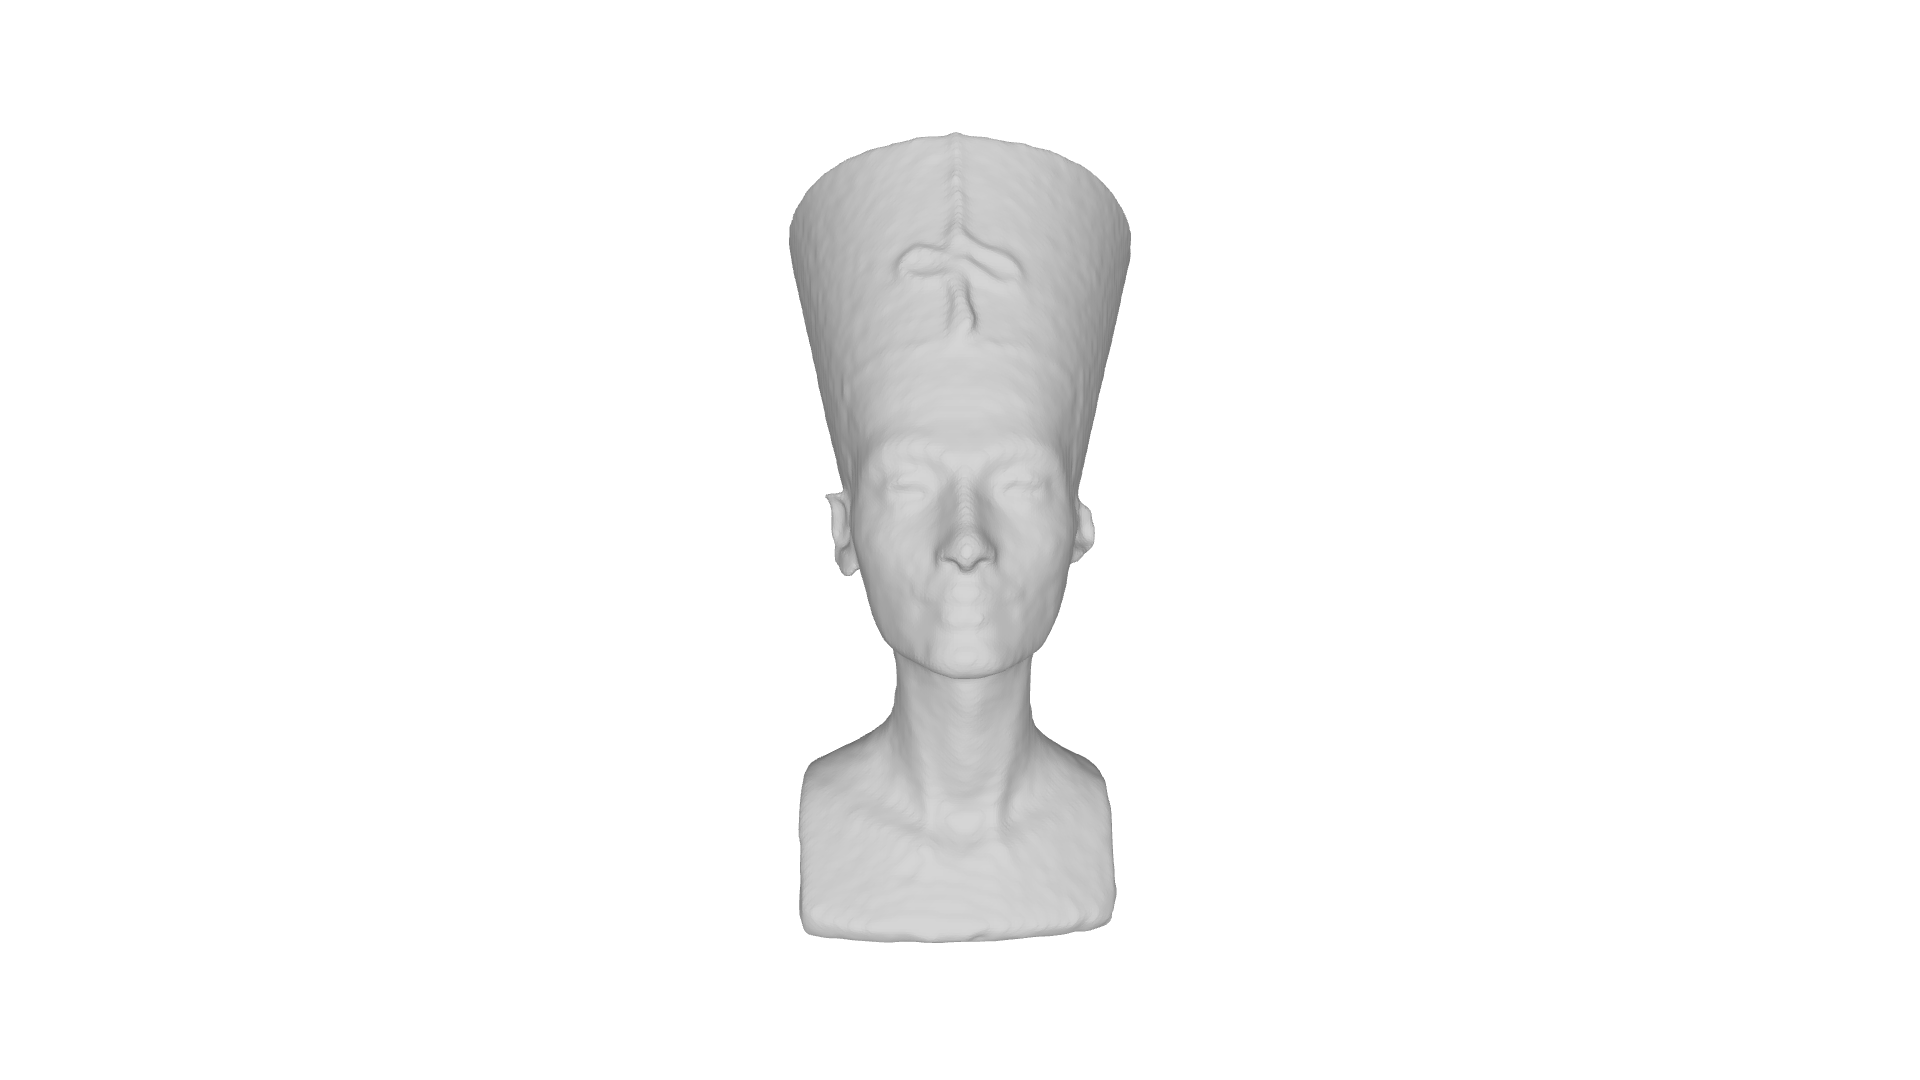
\includegraphics[width=\textwidth]{Figures/results/nefertiti_wire.png}
\caption{WIRE (0.9525)}
\end{subfigure}
\hfill
\begin{subfigure}[b]{0.24\textwidth}
\centering
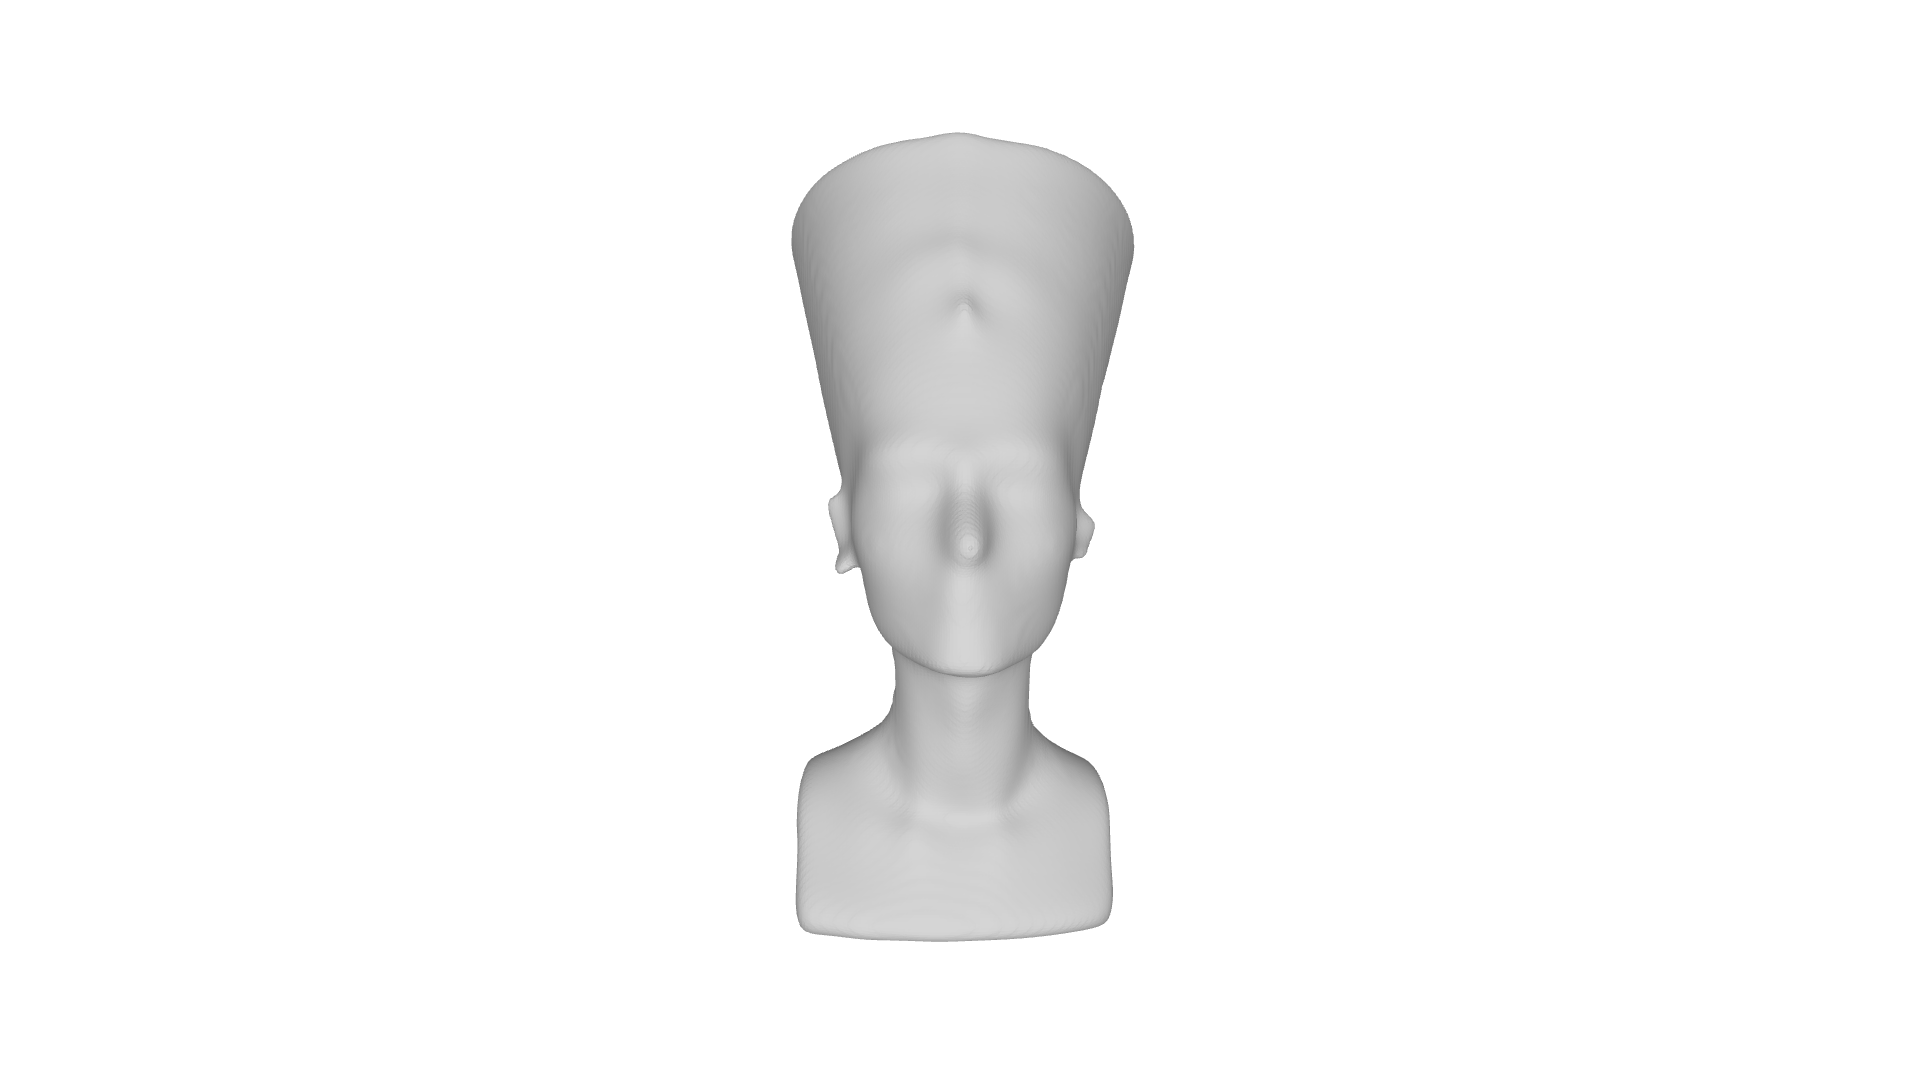
\includegraphics[width=\textwidth]{Figures/results/nefertiti_mfn.png}
\caption{MFN (0.9320)}
\end{subfigure}
\hfill
\begin{subfigure}[b]{0.24\textwidth}
\centering
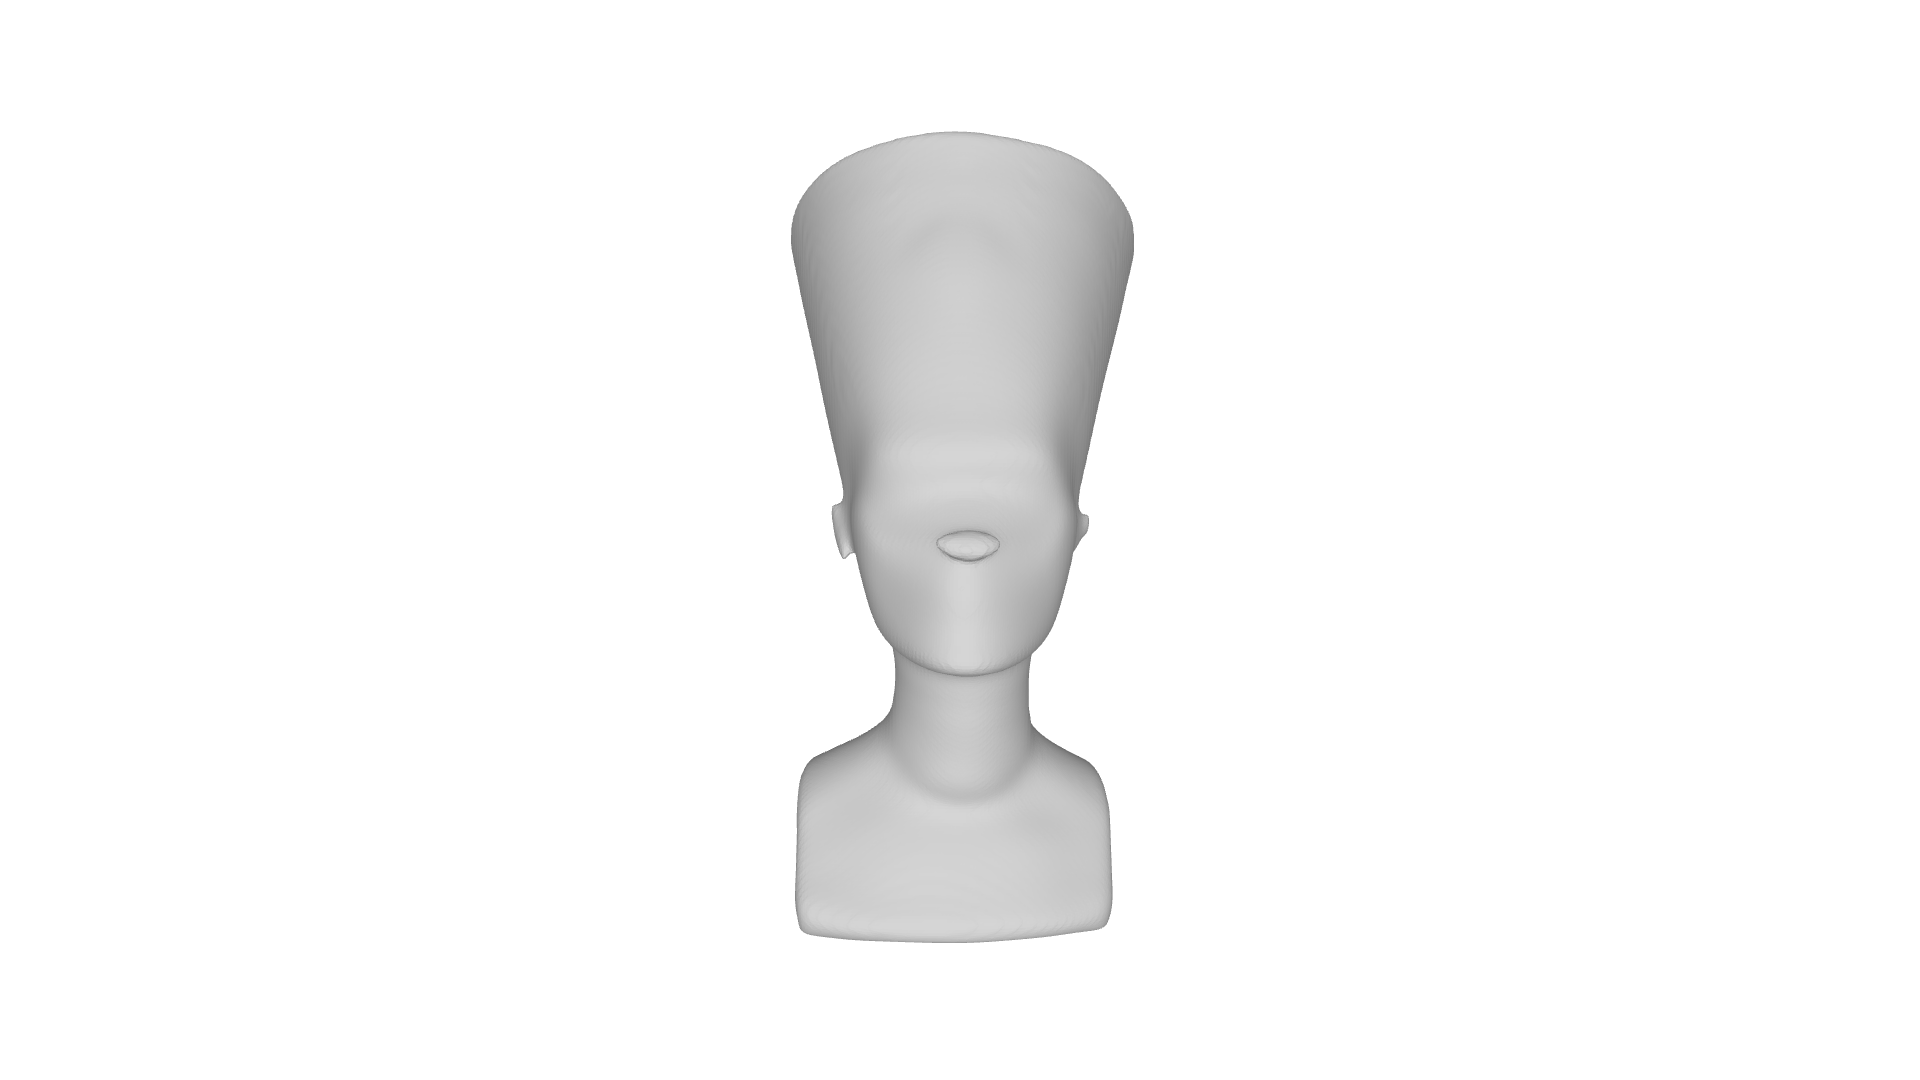
\includegraphics[width=\textwidth]{Figures/results/nefertiti_gauss.png}
\caption{GAUSS (0.9148)}
\end{subfigure}
\caption{Complete visual comparison of all eight INR methods on the Nefertiti bust; the value under each is the four-seed mean evaluation IoU. Methods are rendered from the same viewpoint with consistent lighting and resolution ($1920 \times 1080$). The six higher-scoring reconstructions are hard to tell apart by eye, even though the metrics place Fourier Features and INCODE a clear tier above the rest; the visible differences appear only in the trailing pair, MFN and GAUSS.}
\label{fig:all_methods}
\end{figure}

Two observations follow from the grid. First, the six higher-scoring reconstructions are hard to tell apart by eye, even though the metrics place Fourier Features and INCODE a clear tier above the other four: at this level of quality a one-point IoU difference is not visually obvious, which is why the quantitative separation, not the renders, carries the ranking. Second, the visible differences are confined to the trailing pair: MFN and GAUSS visibly smooth the geometry away, matching their position well below the rest of the field.

\section{Analysis by Architectural Properties}
\label{sec:properties}

\subsection{Frequency Compactness Does Not Survive a Sensitivity Check}

Following the taxonomy in Chapter~\ref{ch:background}, we group methods by whether they possess frequency compactness (FINER, INCODE, GAUSS, WIRE) or not (SIREN, Fourier Features, FR, MFN) and compare group means.

Using the seed-mean IoU, the frequency-compact group averages 0.9473 against 0.9530 for the others: a 0.57 percentage point advantage for the methods \emph{lacking} frequency compactness. Taken alone, this would be read as weak evidence against the property mattering for 3D occupancy.

That reading is not stable, and it is worth showing why, because the instability is the real finding. Dropping GAUSS --- the single weakest run, and a frequency-compact one --- raises the compact group's mean to 0.9581 and reverses the comparison to a 0.51 point advantage \emph{for} frequency compactness. Removing one method of eight, chosen on a defensible ground (it is a clear outlier that fails to fit its own training data), flips the sign of the conclusion. The top-tier result points the same way: the two best methods are one compact (INCODE) and one not (Fourier Features), so the property does not separate the winners from the field either.

A grouped mean over four methods per side is therefore not a sound basis for ranking architectural properties on this task. The sign of the effect is smaller than the influence of any single method, and nothing in the grouped statistic itself signals that fragility. We report it as a negative methodological result: on this evidence, frequency compactness neither predicts the best methods nor survives a leave-one-out check, and establishing whether it matters at all would require many more methods per group, not merely more seeds.

\subsection{Interaction with Adaptivity}

Adaptivity fares slightly better but is still only suggestive. Among frequency-compact methods, those with adaptivity (FINER, INCODE) average 0.9609 against 0.9336 for the non-adaptive pair (GAUSS, WIRE), a gap of 2.7 percentage points that is stable under the seeds. This is consistent with adaptive frequency allocation being useful --- but with two methods per group it rests largely on INCODE being strong and GAUSS weak, and cannot be separated from other differences between those particular methods.

Adaptivity alone certainly does not determine the outcome. FR possesses adaptivity but lacks frequency compactness and lands mid-field; GAUSS lacks adaptivity and places last. Both observations are compatible with a wide range of explanations, including the eight-fold difference in parameter counts across methods discussed in Section~\ref{sec:setup}.

\section{Computational Efficiency}

Training cost is remarkably uniform. Averaged over seeds, seven of the eight methods complete 500 epochs within a narrow band --- roughly 2800 to 3000 seconds (about 47--50 minutes). Only WIRE stands apart at about 4100 seconds (69 minutes), some 45\% slower than the fastest, for the reasons given in Chapter~\ref{ch:implementation}: its complex-valued weights double both storage and arithmetic.

For this workload, then, training time is not a meaningful basis for choosing between methods, with the single exception of avoiding WIRE when compute is constrained. It is worth noting that the two most accurate methods, Fourier Features and INCODE, are also among the faster ones, so the top tier carries no efficiency penalty.

\section{Training Dynamics}
\label{sec:dynamics}

The gap between final training IoU and evaluation IoU separates the methods into distinct regimes, and this split is more informative than the ranking itself. The pattern is consistent across seeds; representative values are quoted below.

Three methods fit the training data essentially perfectly and lose ground at evaluation: SIREN and WIRE both reach a training IoU of 1.0000 while evaluating around 0.956 and 0.953, and FR reaches 0.998 while evaluating at 0.956. Gaps of 4 to 5 points indicate these networks are partly memorizing point labels. This is a direct consequence of the fixed dataset described in Chapter~\ref{ch:methodology}: because the same 450,000 points are revisited every epoch, nothing prevents a sufficiently expressive network from fitting them individually.

Two methods show the opposite behaviour. MFN reaches a training IoU of only about 0.938 and GAUSS only about 0.91 --- in the latter case, essentially equal to or \emph{below} its evaluation IoU. These methods are not oversmoothing at evaluation time; they never fit the training data in the first place. Their weakness is an optimization failure, consistent with both requiring learning-rate overrides to converge at all, and with GAUSS's large seed-to-seed variance.

INCODE and FINER sit between these regimes, with gaps under one point. They neither memorize nor underfit, which is the most plausible explanation for INCODE reaching the top tier. Fourier Features is intermediate, with a gap of about 2.6 points (train $\approx 0.989$, eval $0.9677$) --- larger than INCODE's but well short of the memorizing group, and evidently no barrier to its top-tier accuracy.

The regimes correspond only loosely to final performance --- WIRE memorizes yet lands mid-field, and the two methods with the healthiest gaps (INCODE, FINER) span nearly the full range of the leading group. The train--eval gap explains \emph{how} a method fails, but does not by itself order the field.

\section{Failure Mode Characterization}

\subsection{GAUSS and MFN: Optimization Failure, Not Oversmoothing}

It would be natural to attribute GAUSS's oversmoothed reconstruction (Fig.~\ref{fig:gauss}) to the limited frequency coverage of its rapidly decaying activation, and MFN's weakness to its multiplicative composition. The training IoUs reported above rule this out: a network that cannot fit data it has already seen has not shown that it \emph{could not} represent the target function, only that this optimizer at this learning rate did not find the parameters. Separating the two would require a learning-rate sweep per method, which our fixed protocol excluded --- an exclusion that disadvantages precisely the methods most sensitive to it.

\subsection{Frequency Scale: A Single-Parameter Ablation}
\label{sec:fourier_ablation}

The Fourier Features encoding is governed by two separate parameters: the number of random frequencies $m$, which sets the width of the encoded input, and the scale $\sigma$, which controls how high those frequencies reach. Only $\sigma$ affects frequency content. Because we ran this architecture at both $\sigma = 1.0$ and $\sigma = 10.0$ with everything else held fixed, the pair forms a controlled ablation on frequency scale --- the only such comparison in our results, and the largest effect we measured from any single hyperparameter.

\begin{table}[htbp]
\centering
\caption{Effect of the frequency scale $\sigma$ on Fourier Features, with all other settings held fixed ($m = 256$, 4 hidden layers, 500 epochs).}
\label{tab:sigma_ablation}
\begin{tabular}{lccccc}
\toprule
$\sigma$ & \textbf{Train IoU} & \textbf{Eval IoU} & \textbf{Gap} & \textbf{Chamfer-L1} & \textbf{Normal Cons.} \\
\midrule
1.0  & 0.9892 & \textbf{0.9632} & 0.0260 & \textbf{0.010973} & \textbf{0.9809} \\
10.0 & 1.0000 & 0.7966 & 0.2034 & 0.051407 & 0.6542 \\
\bottomrule
\end{tabular}
\end{table}

\begin{figure}[htbp]
\centering
\begin{subfigure}[b]{0.48\textwidth}
\centering
% NOTE: requires the sigma=1.0 render (see Fig. 5.2 note).
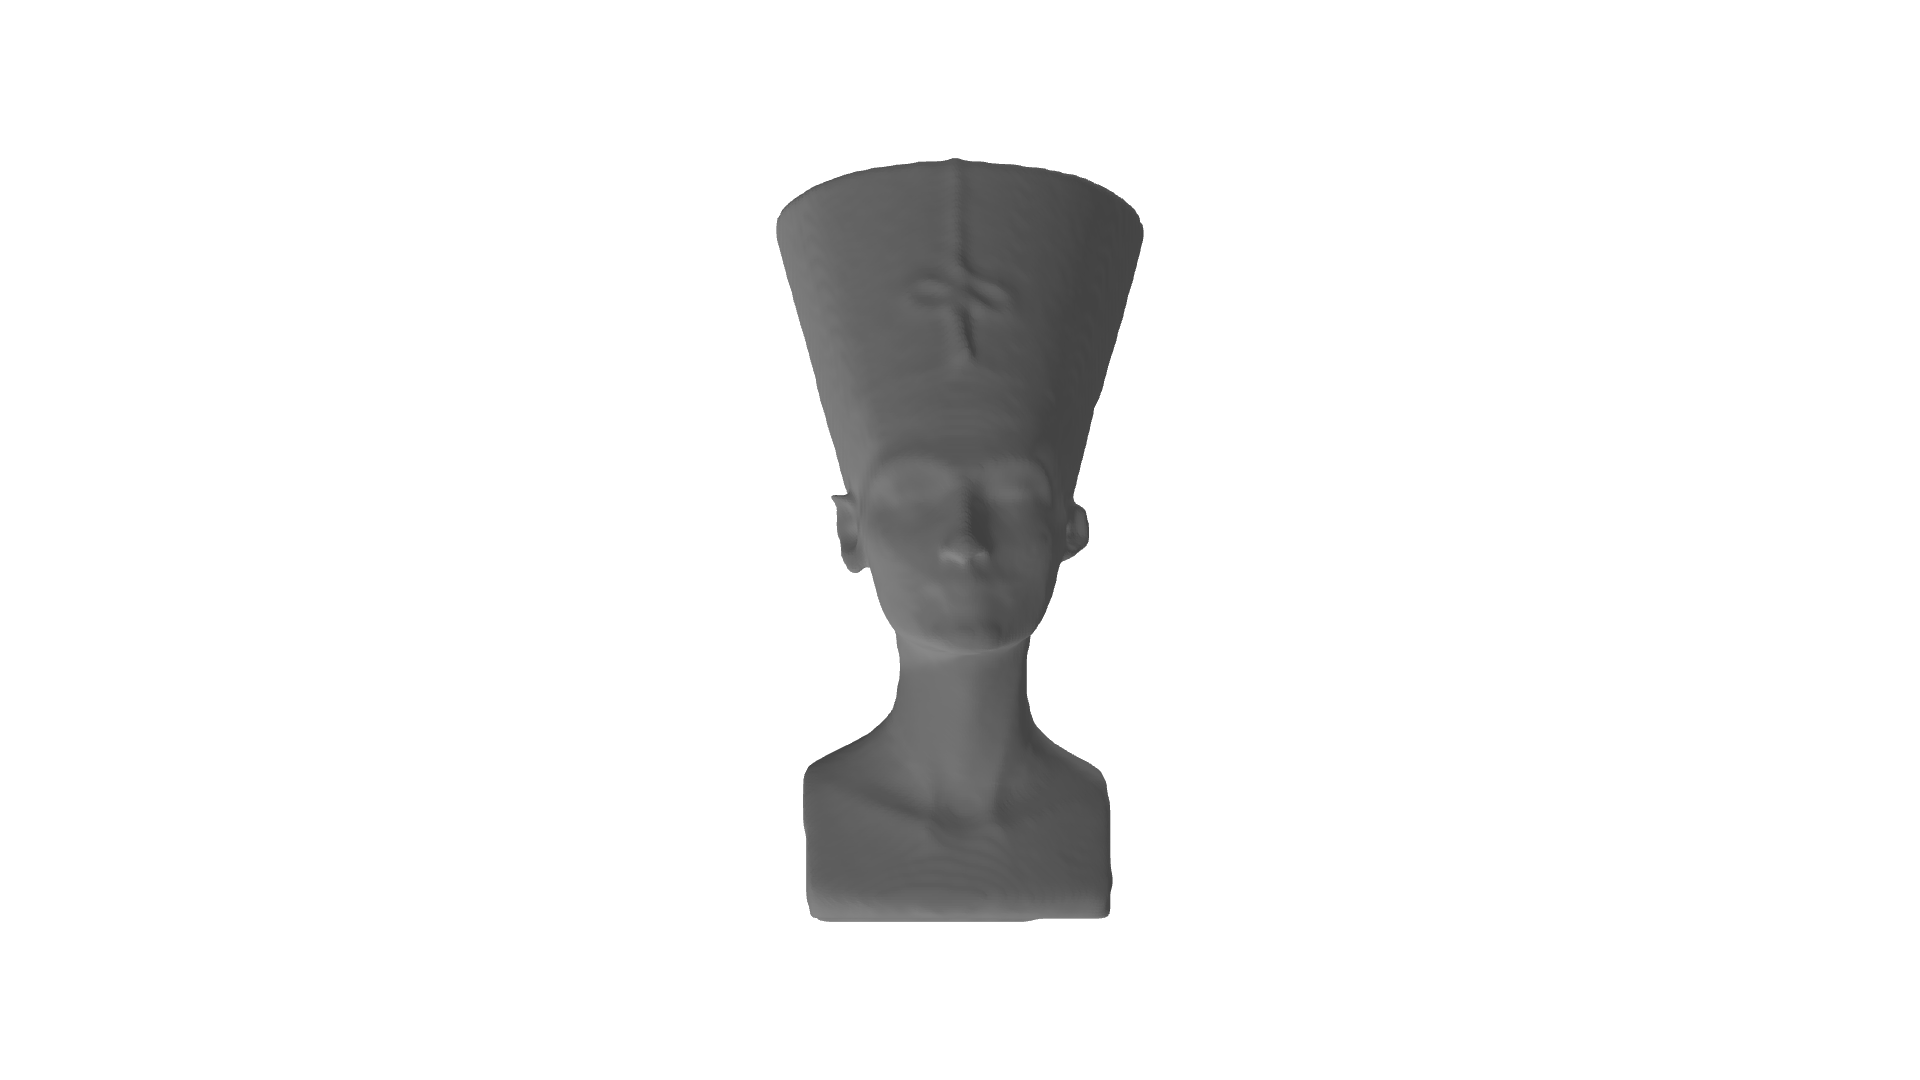
\includegraphics[width=\textwidth]{Figures/results/nefertiti_fourier.png}
\caption{$\sigma = 1.0$ (Eval IoU: 0.9632)}
\label{fig:fourier_s1}
\end{subfigure}
\hfill
\begin{subfigure}[b]{0.48\textwidth}
\centering
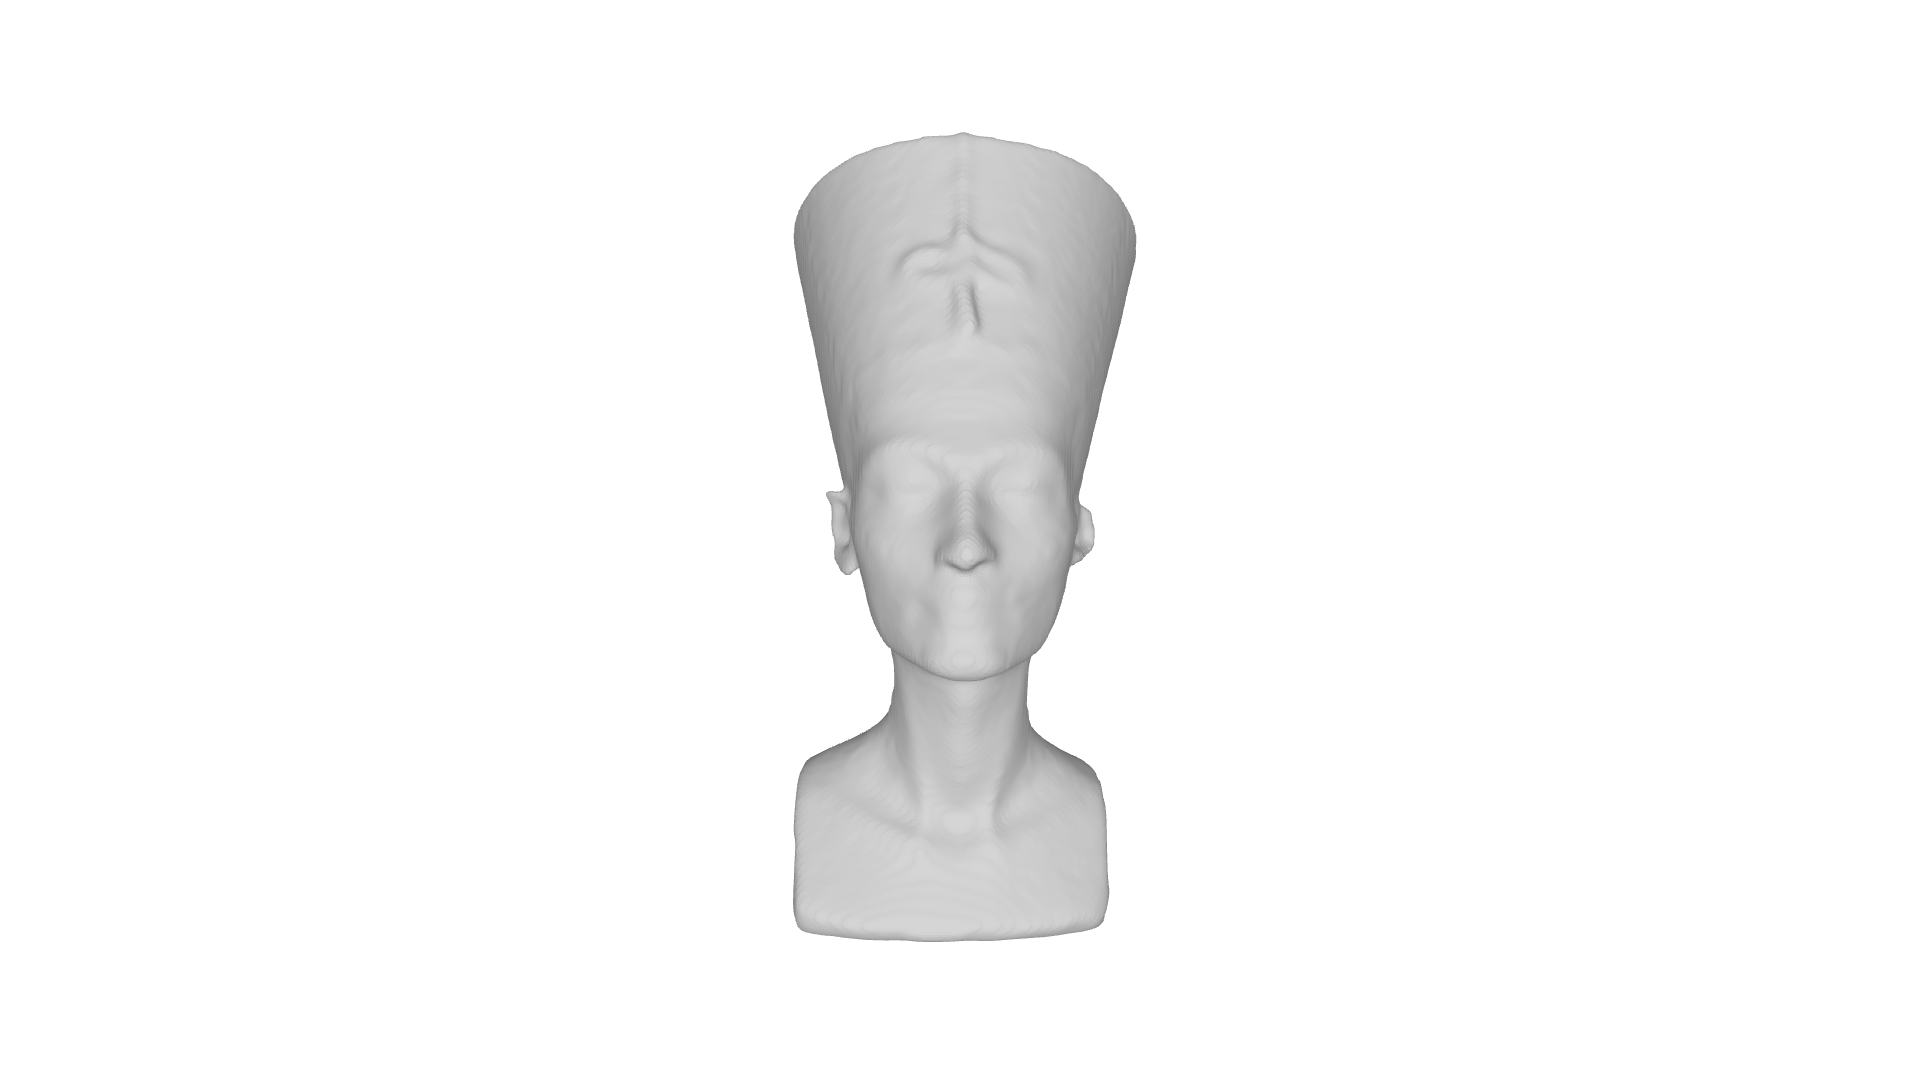
\includegraphics[width=\textwidth]{Figures/results/nefertiti_fourier_sigma10.png}
\caption{$\sigma = 10.0$ (Eval IoU: 0.7966)}
\label{fig:fourier_s10}
\end{subfigure}
\caption{Effect of the frequency scale $\sigma$ on Fourier Features, with all other settings identical. At $\sigma = 10.0$ the reconstruction is distorted rather than smoothed: the face is melted and asymmetric, the eye sockets are hollowed out, the mouth is lost, and wave-like ripples run across the crown and shoulders. These ripples are the signature of an encoding oscillating between correctly classified training points. The same architecture at $\sigma = 1.0$ is competitive with the best method tested.}
\label{fig:sigma_ablation}
\end{figure}

Raising $\sigma$ by one order of magnitude costs 16.7 points of evaluation IoU while \emph{improving} training IoU to a perfect 1.0000. Chamfer-L1 degrades by a factor of nearly five and normal consistency collapses from 0.9809 to 0.6542. At $\sigma = 10.0$ the encoding samples frequencies far above anything present in the geometry, and the network reproduces its training points while oscillating between them; at $\sigma = 1.0$ the same architecture is the joint-best method we tested. (The $\sigma = 1.0$ values in Table~\ref{tab:sigma_ablation} are from the single run matched to the $\sigma = 10.0$ run; over four seeds this configuration averages 0.9677, Table~\ref{tab:seed_results}.)

Three things make this worth reporting. The effect dwarfs every difference between architectures in this study: 16.7 points, an order of magnitude larger than the roughly 1.1-point gap separating the top tier from the middle group, and larger still than any difference within a tier. It is entirely invisible in the training signal, which improves as the model gets worse, so any workflow monitoring only training loss would have shipped the failed configuration. And it shows that a conclusion about \emph{architectures} can be dominated by a single hyperparameter within one of them --- the same fragility seen in the property analysis of Section~\ref{sec:properties}. None of this is evidence against random Fourier features, which are well established~\cite{tancik2020fourier}; it is evidence that the frequency scale must be matched to the target geometry.

\section{Summary of Experimental Findings}

\begin{itemize}
    \item \textbf{Two methods form a distinct top tier.} Over four seeds, Fourier Features ($0.9677 \pm 0.0009$) and INCODE ($0.9674 \pm 0.0022$) are indistinguishable from each other but significantly ahead of every other method (Holm-corrected Welch tests, all $p \le 0.001$); a middle group of SIREN, FR, FINER, and WIRE sits about 1.1 points below. A single run had missed this, placing INCODE first in a six-way near-tie.

    \item \textbf{Two methods are clearly weaker, for optimization not representational reasons.} MFN ($0.9320$) and GAUSS ($0.9148$) trail by 2--4 further points, but both fail on the training set itself, needed learning-rate overrides, and (GAUSS especially) show large seed variance.

    \item \textbf{One hyperparameter outweighs every architectural difference.} Changing the Fourier frequency scale from $\sigma = 1.0$ to $\sigma = 10.0$ costs 16.7 IoU points --- an order of magnitude more than any gap between architectures --- while improving training IoU to 1.0000.

    \item \textbf{The property analysis is not robust.} The frequency-compactness advantage flips sign when the single weakest method is removed, and the top tier pairs one compact method with one non-compact; grouped means do not predict the winners.

    \item \textbf{No method resolves the fine detail the mesh was chosen to test.} Even the best reconstruction loses the headdress band and most of the crown ornament, invisible in an IoU dominated by interior volume. Compute cost does not discriminate either: only WIRE is materially slower (45\%), and the top tier carries no efficiency penalty.
\end{itemize}
